 
\documentclass[preview]{standalone}
%\usepackage{prelude}

%%%%%%%%%%%%%%%%%%%%%%%%%%%%%%%%%%%% PACKAGES %%%%%%%%%%%%%%%%%%%%%%%%%%%%%%%%%%%%%%%%%%

\usepackage{inputenc,fontenc}
\usepackage[a4paper,margin=3cm]{geometry}
\usepackage[english]{babel}
%\usepackage[german]{babel}
%\usepackage[fixlanguage]{babelbib}


\usepackage{bbold}
\usepackage{amsthm}
\usepackage{amsmath}
\usepackage{amssymb} % doteqdot
\usepackage[dvipsnames]{xcolor}
\usepackage{standalone}
\usepackage{tikz}[mode=buildnew]
\usepackage{cite}
\usepackage{xspace}
\usepackage{relsize}
\usepackage{mathtools} % mathclap
%\usepackage{MnSymbol}
\usepackage{hyperref}
\usepackage{url}
\usepackage{listings} % for code
\usepackage[T1]{fontenc} %<
\hypersetup{
	colorlinks,
	citecolor=black,
	filecolor=black,
	linkcolor=black,
	urlcolor=black
}
\usepackage{pgfplots}
\pgfplotsset{compat=1.18}
%\usepackage{courier} %% Sets font for listing as Courier. But also for url and texttt!
\usepackage{listings, xcolor}
\usepackage{graphicx}
\usepackage{subcaption}

\usetikzlibrary{calc}
%\usepackage{xparse} % \newDocumentCommand for multiple optional arguments
%\usepackage{titlecaps}



%%%%%%%%%%%%%%%%%%%%%%%%%%%%%%%%%%%% THEOREMSTYLES %%%%%%%%%%%%%%%%%%%%%%%%%%%%%%%%%%

\theoremstyle{definition}
\newtheorem{definition}{Definition}[section]
\newtheorem{exmp}{Beispiel}[section]
%\AfterEndEnvironment{definition}{\noindent\ignorespaces}

\theoremstyle{theorem}
\newtheorem{theorem}{Satz}[section]
\newtheorem{proposition}{Proposition}[section]
%\AfterEndEnvironment{theorem}{\noindent\ignorespaces}

\theoremstyle{korollary}
\newtheorem{korollary}{Korollar}[section]
%\AfterEndEnvironment{korollary}{\noindent\ignorespaces}


\tikzset{
	mstate/.style={draw, circle, minimum size=.94cm}, 
	gstate/.style={draw, rectangle, minimum size=.8cm},
	varstate/.style={draw,rectangle, rounded corners, minimum size=1}, 
	trans/.style={draw, ->, thick},
	bendtrans/.style={draw, ->, thick, bend left=10},
	bendtransr/.style={draw, ->, thick, bend right=10},
	init/.style={initial, initial distance=6pt, initial text=},
	every loop/.style={min distance=5pt, looseness=8},
	>=latex
}
\usetikzlibrary{automata,positioning}

%auto shift/.style={auto=right,->,
%	to path={ let \p1=(\tikztostart),\p2=(\tikztotarget),
%		\n1={atan2(\y2-\y1,\x2-\x1)},\n2={\n1+180}
%		in ($(\tikztostart.{\n1})!1mm!270:(\tikztotarget.{\n2})$) -- 
%		($(\tikztotarget.{\n2})!1mm!90:(\tikztostart.{\n1})$) \tikztonodes}},

%%%%%%%%%%%%%%%%%%%%%%%%%%%%%%%%%%% MY MACROS %%%%%%%%%%%%%%%%%%%%%%%%%%%%%%%%%%%%%%%%%
%formatting
\newcommand{\comment}[2]{{\color{#1}#2}}
\newcommand{\redcomment}[1]{{\color{red}#1}}
\newcommand{\purpcomment}[1]{{\color{pink}#1}}
\newcommand{\bluecomment}[1]{{\color{blue}#1}}
\newcommand{\mt}[1]{\ensuremath{{#1}}\xspace}
\newcommand{\mynewcommand}[2]{\newcommand{#1}{\mt{#2}}} %% currently not used becaue of ide highlighting
\newcommand{\arr}{\mt{\to}}

%model checking terms
\newcommand{\mimicrel}{\mt{\mathcal{R}}}
\newcommand{\bisimeq}{\mt{\;\!\sim\;\!}}
\newcommand{\simorder}{\mt{\;\!\preceq\;\!}}
\newcommand{\simequiv}{\mt{\;\!\simeq\;\!}} %command already defined
\newcommand{\relts}{\mt{\;\!\bullet_{_{\tiny{TS}}}\;\!}}
\newcommand{\rel}{\mt{\;\!\bullet\;\!}}

%own names
\newcommand{\nm}[1]{#1\xspace}
\newcommand{\mdpN}{\nm{MDP}}
\newcommand{\mdpsN}{\nm{MDPs}}
\newcommand{\viewN}{\nm{view}}
\newcommand{\viewNC}{\nm{View}}
\newcommand{\viewsN}{\nm{views}}
\newcommand{\viewsNC}{\nm{Views}}
\newcommand{\grpfctsubN}{\nm{detached grouping function}}
\newcommand{\grpfctsubNC}{\nm{detached grouping function}}
\newcommand{\grpfctsubNCC}{\nm{Detached Grouping Function}}
\newcommand{\grpfctN}{\nm{grouping function}}
\newcommand{\grpfctNC}{\nm{Grouping function}}
\newcommand{\grpfctNCC}{\nm{Grouping Function}}
\newcommand{\grpfctsN}{\nm{grouping functions}}
\newcommand{\grpfctsNC}{\nm{Grouping functions}}
\newcommand{\grpfctsNCC}{\nm{Grouping Functions}}
\newcommand{\stmimicN}{\nm{state-mimic}}
\newcommand{\stmimicsN}{\nm{state-mimics}}
\newcommand{\stmimickingN}{\nm{state-mimicking}}
\newcommand{\stmimickedN}{\nm{state-mimicked}}
%\newcommand{\chosenphtypeNCC}{\nm{Transition System}}
%\newcommand{\chgphNC}{\nm{Transition system}}
%\newcommand{\chgphN}{\nm{transition system}}
%\newcommand{\chgphsNCC}{\nm{Transition Systems}}
%\newcommand{\chgphsNC}{\nm{Transition systems}}
%\newcommand{\chgphsN}{\nm{transition systems}}
\newcommand{\chgphNCC}{\nm{MDP}}
\newcommand{\chgphNC}{\nm{MDP}}
\newcommand{\chgphN}{\nm{MDP}}
\newcommand{\achgphN}{\nm{an MDP}}
\newcommand{\chgphsNCC}{\nm{MDPs}}
\newcommand{\chgphsNC}{\nm{MDPs}}
\newcommand{\chgphsN}{\nm{MDPs}}
\newcommand{\parllcompN}{\nm{parallel composition}}
\newcommand{\parllcompNC}{\nm{Parallel composition}}
\newcommand{\parllcompNCC}{\nm{Parallel Composition}}
\newcommand{\parllcompsN}{\nm{parallel compositions}}
\newcommand{\parllcompsNC}{\nm{Parallel compositions}}
\newcommand{\parllcompsNCC}{\nm{Parallel Compositions}}
\newcommand{\sccN}{\nm{SCC}}
\newcommand{\sccsN}{\nm{SCCs}}
\newcommand{\bsccN}{\nm{BSCC}}
\newcommand{\bsccsN}{\nm{BSCCs}}
\newcommand{\jgrapht}{\nm{jGraphtT}}

\newcommand{\outactident}{\nm{OutActionsIdent}}

%names
\newcommand{\iffN}{\nm{if and only if}}
\newcommand{\tsN}{\nm{TS}}

%% outactions identical
\newcommand{\outactidentstrong}{\nm{strong}}
\newcommand{\outactidentweak}{\nm{weak}}

% CORE DEFINITIONS
\newcommand{\grpfct}[1][\viewppty]{\mt{F_{#1}}}
\newcommand{\grpfctsub}[1][\viewppty]{\mt{\tilde{F}_{#1}}}
%\newcommand{\grpfctimg}[1]{\mt{{\grpfct}[{#1}]}}
%\newcommand{\fctimg}[2]{\mt{{#1}[{#2}]}}
\newcommand{\eqrelview}{\mt{R}}
\newcommand{\eqclassv}[1][\state]{\mt{\eqclass{#1}{\eqrelview}}}
\newcommand{\eqclasssetv}[1][\states]{\mt{{#1}/\eqrelview}} %OLD: \bigcup_{\state \in \states} \eqclassv
\newcommand{\viewid}{\mt{\mdp}}
\newcommand{\view}[1][\viewppty]{\mt{\viewid_{#1}}}
\newcommand{\imggrp}{\mt{\arbset}}
\newcommand{\imggrpsub}{\mt{X}}
\newcommand{\viewppty}{\mt{\theta}}
\newcommand{\pll}{\mt{\;\!\pllpure\;\!}}
\newcommand{\pllrev}{\mt{\pllpure^{-1}}}
\newcommand{\pllpure}{\mt{||}}
\newcommand{\compselectset}{\mt{Z}}
\newcommand{\compselectpure}{\mt{\pllpure_\compselectset}}
\newcommand{\compselect}{\mt{\;\pllpure_\compselectset\;}}
\newcommand{\remstates}{\mt{\bigcup_{\state \in \states \setminus \states_1}\{\{\state\}\}}}
\newcommand{\nogroupstates}[1][\states_2]{\mt{\bigcup_{\state \in \states \setminus {#1}}\{\{\state\}\}}}
\newcommand{\remelem}{\mt{\bullet}}
\newcommand{\nogroupset}{\mt{\xi}}
\newcommand{\remset}{\mt{\{\remelem\}}}
\newcommand{\gfctpll}{\mt{\grpfct[\pll]}}
\newcommand{\group}{\mt{\top}}
\newcommand{\imggrpbinview}{\mt{\{\remelem, \notppty\}}}
\newcommand{\viewappset}{\mt{\tilde{\states}}}
\newcommand{\hasppty}{\mt{\top}}
\newcommand{\notppty}{\mt{\bot}}
\newcommand{\disregardelem}{\mt{\Delta}}
\newcommand{\disregardelements}{\mt{{\disregardelem_1, \dots, \disregardelem_n}}}



%\newcommand{\mdp}{def}\mdp
%\newcommand{\mdpdef}



% EXAMPLE VIEWS
\newcommand{\pptyatomicprops}{\mt{\atomicprops}}
\newcommand{\pptyinitstates}{\mt{\initstates}}
\newcommand{\pptyinactsetsize}{\mt{|\inacts(\state)|}}
\newcommand{\pptyhasoutact}{\mt{\exists\outact}}
\newcommand{\pptyminoutact}[2]{\mt{#1\leq#2}}
\newcommand{\pptymaxoutact}[2]{\mt{#2\leq#1}}
\newcommand{\pptyspanoutact}[3]{\mt{#1\leq#2\leq#3}}
\newcommand{\pptyoutactsetsize}{\mt{|\outacts(\state)|}}
\newcommand{\pptyoutactsingle}{\mt{|\outacts(\state)|_1}}
\newcommand{\pptystrongoutactident}{\mt{\outacts(\state)_=}}
\newcommand{\pptyweakoutactident}{\mt{\outacts(\state)_\approx}}
\newcommand{\pptyhasinact}{\mt{\exists\inact}}
\newcommand{\pptymininact}[2]{\mt{#1\leq#2}}
\newcommand{\pptymaxinact}[2]{\mt{#2\leq#1}}
\newcommand{\pptyspaninact}[3]{\mt{#1\leq#2\leq#3}}
\newcommand{\pptyinactsingle}{\mt{|\inacts(\state)|_1}}
\newcommand{\pptystronginactident}{\mt{\inacts(\state)_=}}
\newcommand{\pptyweakinactident}{\mt{\inacts(\state)_\approx}}
\newcommand{\pptyparamvalueseq}{\mt{\var = \varval}}
\newcommand{\pptyparamvaluesneq}{\mt{\var \neq \varval}}
\newcommand{\pptyparamdnf}{\mt{VarDNF}}
\newcommand{\pptyparamcnf}{\mt{VarCNF}}
\newcommand{\pptyparamvalueseqopt}{\mt{\var = \varval}}
\newcommand{\pptyparamvalident}{\mt{Var:\varval}}
\newcommand{\pptydistance}{\mt{\distpath}}
\newcommand{\pptydistancerev}{\mt{\distpathrev}}
\newcommand{\pptydistancebi}{\mt{\distpathbi}}
\newcommand{\pptyhascycle}{\mt{\exists\cycle}}
\newcommand{\pptyexactactcycle}{\mt{\{\cycle_{\action,n}\}}}
\newcommand{\pptycycleset}{\mt{\cup{\{\state\}_\cycle}}}
\newcommand{\pptyexactcycle}{\mt{\{\cycle_n\}}}
\newcommand{\pptyscc}{\mt{scc}}
\newcommand{\pptybscc}{\mt{bscc}}
\newcommand{\pptyprop}{\mt{\redcomment{?}}}
\newcommand{\pptyident}{id}


\newcommand{\gfctatomicprops}{\mt{\grpfct[\pptyatomicprops]}}
\newcommand{\gfctinitstates}{\mt{\grpfct[\pptyinitstates]^\hasppty}}
\newcommand{\gfcthasoutaction}{\mt{\grpfct[\pptyhasoutact]^\hasppty}}
\newcommand{\gfctminoutaction}{\mt{\grpfct[\pptyminoutact{\numoutact}{\outact}]^\hasppty}}
\newcommand{\gfctmaxoutaction}{\mt{\grpfct[\pptymaxoutact{\numoutact}{\outact}]^\hasppty}}
\newcommand{\gfctspanoutaction}{\mt{\grpfct[\pptyspanoutact{\numoutactb}{\outact}{\numoutact}]^\hasppty}}
\newcommand{\gfctoutactsetsize}{\mt{\grpfct[\pptyoutactsetsize]}}
\newcommand{\gfctoutactsingle}{\mt{\grpfct[\pptyoutactsingle]^\notppty}}
\newcommand{\gfctstrongoutactident}{\mt{\grpfct[\pptystrongoutactident]}}
\newcommand{\gfctweakoutactident}{\mt{\grpfct[\pptyweakoutactident]}}
\newcommand{\gfcthasinaction}{\mt{\grpfct[\pptyhasinact]^\hasppty}}
\newcommand{\gfctmininaction}{\mt{\grpfct[\pptymininact{\numinact}{\inact}]^\hasppty}}
\newcommand{\gfctmaxinaction}{\mt{\grpfct[\pptymaxinact{\numinact}{\inact}]^\hasppty}}
\newcommand{\gfctspaninaction}{\mt{\grpfct[\pptyspaninact{\numinactb}{\inact}{\numinact}]^\hasppty}}
\newcommand{\gfctinactsetsize}{\mt{\grpfct[\pptyinactsetsize]}}
\newcommand{\gfctinactsingle}{\mt{\grpfct[\pptyinactsingle]^\notppty}}
\newcommand{\gfctstronginactident}{\mt{\grpfct[\pptystronginactident]}}
\newcommand{\gfctweakinactident}{\mt{\grpfct[\pptyweakinactident]}}
\newcommand{\gfctparamvalueseq}{\mt{\grpfct[\pptyparamvalueseq]^\hasppty}}
\newcommand{\gfctparamvaluesneq}{\mt{\grpfct[\pptyparamvaluesneq]^\hasppty}}
\newcommand{\gfctparamdnf}{\mt{\grpfct[\pptyparamdnf]^\hasppty}}
\newcommand{\gfctparamcnf}{\mt{\grpfct[\pptyparamcnf]^\hasppty}}
\newcommand{\gfctparamvalueseqopt}{\mt{\pptyparamvalueseqopt}}
\newcommand{\gfctparamvalident}{\mt{\grpfct[\pptyparamvalident]}}
\newcommand{\gfctdistance}{\mt{\grpfct[\pptydistance]}}
\newcommand{\gfctdistancerev}{\mt{\grpfct[\pptydistancerev]}}
\newcommand{\gfctdistancebi}{\mt{\grpfct[\pptydistancebi]}}
\newcommand{\gfcthascycle}{\mt{\grpfct[\pptyhascycle]}}
\newcommand{\gfctexactcycle}{\mt{\grpfct[\pptyexactcycle]}}
\newcommand{\gfctcycleset}{\mt{\grpfct[\pptycycleset]}}
\newcommand{\gfctexactactcycle}{\mt{\grpfct[\pptyexactactcycle]}}
\newcommand{\gfctscc}{\mt{\grpfct[\pptyscc]}}
\newcommand{\gfctbscc}{\mt{\grpfct[\pptybscc]}}
\newcommand{\gfctprop}{\mt{\grpfct[\pptyprop]}}
\newcommand{\gfctident}{\mt{\grpfct[\pptyident]}}

\newcommand{\gfctsubatomicprops}{\mt{\grpfctsub[\pptyatomicprops]}}
\newcommand{\gfctsubinitstates}{\mt{\grpfctsub[\pptyinitstates]^\hasppty}}
\newcommand{\gfctsubhasoutaction}{\mt{\grpfctsub[\pptyhasoutact]^\hasppty}}
\newcommand{\gfctsubminoutaction}{\mt{\grpfctsub[\pptyminoutact{\numoutact}{\outact}]^\hasppty}}
\newcommand{\gfctsubmaxoutaction}{\mt{\grpfctsub[\pptymaxoutact{\numoutact}{\outact}]^\hasppty}}
\newcommand{\gfctsubspanoutaction}{\mt{\grpfctsub[\pptyspanoutact{\numoutactb}{\outact}{\numoutact}]^\hasppty}}
\newcommand{\gfctsuboutactsetsize}{\mt{\grpfctsub[\pptyoutactsetsize]}}
\newcommand{\gfctsuboutactsingle}{\mt{\grpfctsub[\pptyoutactsingle]^\notppty}}
\newcommand{\gfctsubstrongoutactident}{\mt{\grpfctsub[\pptystrongoutactident]^\hasppty}}
\newcommand{\gfctsubweakoutactident}{\mt{\grpfctsub[\pptyweakoutactident]^\hasppty}}
\newcommand{\gfctsubhasinaction}{\mt{\grpfctsub[\pptyhasinact]}}
\newcommand{\gfctsubmininaction}{\mt{\grpfctsub[\pptymininact{\numinact}{\inact}]}}
\newcommand{\gfctsubmaxinaction}{\mt{\grpfctsub[\pptymaxinact{\numinact}{\inact}]}}
\newcommand{\gfctsubspaninaction}{\mt{\grpfctsub[\pptyspaninact{\numinactb}{\inact}{\numinact}]}}
\newcommand{\gfctsubinactsetsize}{\mt{\grpfctsub[\pptyinactsetsize]^\hasppty}}
\newcommand{\gfctsubinactsingle}{\mt{\grpfctsub[\pptyinactsingle]^\notppty}}
\newcommand{\gfctsubstronginactident}{\mt{\grpfctsub[\pptystronginactident]}}
\newcommand{\gfctsubweakinactident}{\mt{\grpfctsub[\pptyweakinactident]}}
\newcommand{\gfctsubparamvalueseq}{\mt{\grpfctsub[\pptyparamvalueseq]^\hasppty}}
\newcommand{\gfctsubparamvaluesneq}{\mt{\grpfctsub[\pptyparamvaluesneq]^\hasppty}}
\newcommand{\gfctsubparamdnf}{\mt{\grpfctsub[\pptyparamdnf]^\hasppty}}
\newcommand{\gfctsubparamcnf}{\mt{\grpfctsub[\pptyparamcnf]^\hasppty}}
\newcommand{\gfctsubparamvalueseqopt}{\mt{\pptyparamvalueseqopt}}
\newcommand{\gfctsubparamvalident}{\mt{\grpfctsub[\pptyparamvalident]}}
\newcommand{\gfctsubdistance}{\mt{\grpfctsub[\pptydistance]}}
\newcommand{\gfctsubdistancerev}{\mt{\grpfctsub[\pptydistancerev]}}
\newcommand{\gfctsubdistancebi}{\mt{\grpfctsub[\pptydistancebi]}}
\newcommand{\gfctsubhascycle}{\mt{\grpfctsub[\pptyhascycle]^\hasppty}}
\newcommand{\gfctsubexactcycle}{\mt{\grpfctsub[\pptyexactcycle]}}
\newcommand{\gfctsubcycleset}{\mt{\grpfctsub[\pptycycleset]}}
\newcommand{\gfctsubexactactcycle}{\mt{\grpfctsub[\pptyexactactcycle]}}
\newcommand{\gfctsubscc}{\mt{\grpfctsub[\pptyscc]}}
\newcommand{\gfctsubbscc}{\mt{\grpfctsub[\pptybscc]}}
\newcommand{\gfctsubprop}{\mt{\grpfctsub[\pptyprop]}}
\newcommand{\gfctsubident}{\mt{\grpfctsub[\pptyident]}}


\newcommand{\viewatomicprops}{\mt{\view[\pptyatomicprops]}}
\newcommand{\viewinitstates}{\mt{\view[\pptyinitstates]^\hasppty}}
\newcommand{\viewhasoutaction}{\mt{\view[\pptyhasoutact]^\hasppty}}
\newcommand{\viewminoutaction}{\mt{\view[\pptyminoutact{\numoutact}{\outact}]^\hasppty}}
\newcommand{\viewmaxoutaction}{\mt{\view[\pptymaxoutact{\numoutact}{\outact}]^\hasppty}}
\newcommand{\viewspanoutaction}{\mt{\view[\pptyspanoutact{\numoutactb}{\outact}{\numoutact}]^\hasppty}}
\newcommand{\viewoutactsetsize}{\mt{\view[\pptyoutactsetsize]}}
\newcommand{\viewoutactsingle}{\mt{\view[\pptyoutactsingle]^\notppty}}
\newcommand{\viewstrongoutactident}{\mt{\view[\pptystrongoutactident]}}
\newcommand{\viewweakoutactident}{\mt{\view[\pptyweakoutactident]}}
\newcommand{\viewhasinaction}{\mt{\view[\pptyhasinact]^\hasppty}}
\newcommand{\viewmininaction}{\mt{\view[\pptymininact{\numinact}{\inact}]^\hasppty}}
\newcommand{\viewmaxinaction}{\mt{\view[\pptymaxinact{\numinact}{\inact}]^\hasppty}}
\newcommand{\viewspaninaction}{\mt{\view[\pptyspaninact{\numinactb}{\inact}{\numinact}]^\hasppty}}
\newcommand{\viewinactsetsize}{\mt{\view[\pptyinactsetsize]}}
\newcommand{\viewinactsingle}{\mt{\view[\pptyinactsingle]^\notppty}}
\newcommand{\viewstronginactident}{\mt{\view[\pptystronginactident]}}
\newcommand{\viewweakinactident}{\mt{\view[\pptyweakinactident]}}
\newcommand{\viewparamvalueseq}{\mt{\view[\pptyparamvalueseq]}}
\newcommand{\viewparamvaluesneq}{\mt{\view[\pptyparamvaluesneq]}}
\newcommand{\viewparamdnf}{\mt{\view[\pptyparamdnf]^\hasppty}}
\newcommand{\viewparamcnf}{\mt{\view[\pptyparamcnf]^\hasppty}}
\newcommand{\viewparamvalueseqopt}{\mt{\pptyparamvalueseqopt}}
\newcommand{\viewparamvalident}{\mt{\view[\pptyparamvalident]}}
\newcommand{\viewdistance}{\mt{\view[\pptydistance]}}
\newcommand{\viewdistancerev}{\mt{\view[\pptydistancerev]}}
\newcommand{\viewdistancebi}{\mt{\view[\pptydistancebi]}}
\newcommand{\viewhascycle}{\mt{\view[\pptyhascycle]}}
\newcommand{\viewexactcycle}{\mt{\view[\pptyexactcycle]}}
\newcommand{\viewcycleset}{\mt{\view[\pptycycleset]}}
\newcommand{\viewexactactcycle}{\mt{\view[\pptyexactactcycle]}}
\newcommand{\viewscc}{\mt{\view[\pptyscc]}}
\newcommand{\viewbscc}{\mt{\view[\pptybscc]}}
\newcommand{\viewprop}{\mt{\view[\pptyprop]}}
\newcommand{\viewident}{\mt{\view[\pptyident]}}

%\newcommand{\viewatomicprops}{\mt{\view[\atomicprops]}}
%\newcommand{\viewinitstates}{\mt{\view[\initstates]}}
%\newcommand{\viewhasoutaction}{\mt{\view[\pptyhasoutact]}}
%\newcommand{\viewminoutaction}{\mt{\view[\pptyminoutact{\numoutact}{\outact}]}}
%\newcommand{\viewmaxoutaction}{\mt{\view[\pptymaxoutact{\numoutact}{\outact}]}}
%\newcommand{\viewspanoutaction}{\mt{\view[\pptyspanoutact{\numoutactb}{\outact}{\numoutact}]}}
%\newcommand{\viewoutactsetsize}{\mt{\view[\pptyoutactsetsize]}}
%\newcommand{\viewoutactsingle}{\mt{\view[\pptyoutactsingle]}}
%\newcommand{\viewstrongoutactident}{\mt{\view[\outacts(\state)_=]}}
%\newcommand{\viewweakoutactident}{\mt{\view[\outacts(\state)_\approx]}}
%\newcommand{\viewhasinaction}{\mt{\view[\pptyhasinact]}}
%\newcommand{\viewmininaction}{\mt{\view[\pptymininact{\numinact}{\inact}]}}
%\newcommand{\viewmaxinaction}{\mt{\view[\pptymaxinact{\numinact}{\inact}]}}
%\newcommand{\viewspaninaction}{\mt{\view[\pptyspaninact{\numinactb}{\inact}{\numinact}]}}
%\newcommand{\viewinactsetsize}{\mt{\view[\pptyinactsetsize]}}
%\newcommand{\viewinactsingle}{\mt{\view[\pptyinactsingle]}}
%\newcommand{\viewstronginactident}{\mt{\view[\inacts(\state)_=]}}
%\newcommand{\viewweakinactident}{\mt{\view[\inacts(\state)_\approx]}}
%\newcommand{\viewparamvalueseq}{\mt{\view[\var = \varval]}}
%\newcommand{\viewparamvaluesneq}{\mt{\view[\var \neq \varval]}}
%\newcommand{\viewparamdnf}{\mt{\view[VarDNF]}}
%\newcommand{\viewparamcnf}{\mt{\view[VarCNF]}}
%\newcommand{\viewparamvalident}{\mt{\view[\pptyparamvalident]}}
%\newcommand{\viewdistance}{\mt{\view[\pptydistance]}}
%\newcommand{\viewhascycle}{\mt{\view[\exists\cycle]}}
%\newcommand{\viewexactcycle}{\mt{\view[\pptyexactcycle]}}
%\newcommand{\viewcycleset}{\mt{\view[\pptycycleset]}}
%\newcommand{\viewexactactcycle}{\mt{\view[\pptyexactactcycle]}}
%\newcommand{\viewscc}{\mt{\view[scc]}}
%\newcommand{\viewbscc}{\mt{\view[bscc]}}

%actions
\newcommand{\numoutact}{\mt{n}}
\newcommand{\numoutactb}{\mt{m}}
\newcommand{\numinact}{\mt{n}}
\newcommand{\numinactb}{\mt{m}}

\newcommand{\predmaxoutact}[1][\numoutact]{\mt{Q_{\outact\leq#1}(\state,\state_1, \dots, \state_{#1+1})}}
\newcommand{\predminoutact}[1][\numoutact]{\mt{Q_{#1\leq\outact}(\state,\state_1, \dots, \state_{#1})}}
\newcommand{\formoutact}[1][\state]{\mt{C_{#1,\outact}}}
\newcommand{\predmaxinact}[1][\numinact]{\mt{Q_{\inact\leq#1}(\state,\state_1, \dots, \state_{#1+1})}}
\newcommand{\predmininact}[1][\numinact]{\mt{Q_{#1\leq\inact}(\state,\state_1, \dots, \state_{#1})}}

\newcommand{\outact}[1][\action]{\mt{\overrightarrow{#1}}}
\newcommand{\outacts}{\mt{\overrightarrow{\actions}}}
\newcommand{\inact}{\mt{\overleftarrow{\action}}}
\newcommand{\inacts}[1][\action]{\mt{\overleftarrow{#1}}}

%%Parameters
\newcommand{\vars}[1][\mdp]{\mt{V\!ar_{#1}}}
\newcommand{\var}{\mt{x}}
\newcommand{\varstate}[1][]{\mt{\var_{\state#1}}}
\newcommand{\varval}{\mt{a}}
\newcommand{\vareval}[1][\mdp]{\mt{V\!arEval_{#1}}}
\newcommand{\varevalimg}[1][\mdp]{\mt{\vareval[#1][\states,\vars]}}
\newcommand{\varevalimgset}{\mt{\arbset}}
\newcommand{\someparam}{\mt{\tilde{x}}}
\newcommand{\eqorneq}{\mt{\;\doteqdot\;}}
\newcommand{\varstyle}[2]{\mt{\langle#1,#2\rangle}}




%\makeatletter
%\newcommand{\overleftrightsmallarrow}{\mathpalette{\overarrowsmall@\leftrightarrowfill@}}
%\newcommand{\overrightsmallarrow}{\mathpalette{\overarrowsmall@\rightarrowfill@}}
%\newcommand{\overleftsmallarrow}{\mathpalette{\overarrowsmall@\leftarrowfill@}}
%\newcommand{\overarrowsmall@}[3]{%
%	\vbox{%
%		\ialign{%
%			##\crcr
%			#1{\smaller@style{#2}}\crcr
%			\noalign{\nointerlineskip}%
%			$\m@th\hfil#2#3\hfil$\crcr
%		}%
%	}%
%}
%\def\smaller@style#1{%
%	\ifx#1\displaystyle\scriptstyle\else
%	\ifx#1\textstyle\scriptstyle\else
%	\scriptscriptstyle
%	\fi
%	\fi
%}
%\makeatother
%\newcommand{\te}[1]{\overleftrightsmallarrow{#1}}

% Distance
\newcommand{\fctdist}{\mt{distance}}
\newcommand{\fctdistdefault}{\mt{\fctdist(\chgph, \smstates, \grandist)}}
\newcommand{\distval}{\mt{d}}
\newcommand{\grandist}{\mt{n}}
\let\path\oldpath
\newcommand{\path}{\mt{P}}
\newcommand{\pathbi}{\mt{\bar{\path}}}
\newcommand{\pathsecfull}{\mt{(\state_0, \action_0, \state_1, \action_1, \dots, \action_{n}, \state_{n+1})}}
\newcommand{\lenpath}{\mt{len}}
\newcommand{\pfirst}{\mt{first}}
\newcommand{\plast}{\mt{last}}
\newcommand{\pathset}{\mt{\path_\chgph}}
\newcommand{\pathbiset}{\mt{\pathbi_\chgph}}
\newcommand{\distpath}{\mt{\overrightarrow{dist}}}
\newcommand{\distpathrev}{\mt{\overleftarrow{dist}}}
\newcommand{\distpathbi}{\mt{\overline{dist}}}
%Cycles
\newcommand{\cyclesecfull}{\mt{(\state_0, \action_0, \state_1, \action_1, \dots, \action_{n-1}, \state_0)}}
\newcommand{\fctfindcycles}{\mt{findCycles}}
\newcommand{\cycle}{\mt{C}}
\newcommand{\cycleset}{\mt{\cycle_{\mdp, n}}}
\newcommand{\lencycle}{\mt{len}}
% strongly connected components
\newcommand{\scc}{\mt{T}}
\newcommand{\setscc}{\mt{SCC_{\chgph,n}}}
\newcommand{\setbscc}{\mt{BSCC_{\chgph,n}}}

% properties
\newcommand{\propfct}{\mt{f}}

% all Systems
\newcommand{\chgph}{\mt{\mdp}}
\newcommand{\chgphtuple}{\mt{\mdptuple}}
\newcommand{\chgphtupledist}{\mt{\mdptupledist}}

\newcommand{\states}{\mt{S}}
\newcommand{\actions}{\mt{Act}}
\newcommand{\atomicprops}{\mt{AP}}
\newcommand{\labelingfct}{\mt{L}}
\newcommand{\init}{\mt{\initdistrib}} % use MDP % refers to the underlying set
\newcommand{\trans}{\mt{\probtfunc}} % use MDP % refers to the underlying set
\newcommand{\smstates}{\mt{\tilde{\states}}}


\newcommand{\state}{\mt{s}}
\newcommand{\action}{\mt{\alpha}}
\newcommand{\actionb}{\mt{\beta}}
\newcommand{\actionc}{\mt{\gamma}}
\newcommand{\smstate}{\mt{\tilde{\state}}}



% transition sysstems
\newcommand{\ts}{\mt{TS}}
\newcommand{\transitionrel}{\mt{\longrightarrow}}
\newcommand{\initstates}{\mt{I}}
\newcommand{\transitionsystem}{\mt
	{(\states, \actions, \transitionrel, \initstates, \atomicprops, \labelingfct)}
}
\newcommand{\tstupledist}{\mt{(\states', \actions',\transitionrel', \initstates', \labelingfct')}}


%Markov chains and MDP
\newcommand{\mdp}{\mt{\autm}}
\newcommand{\mdptuple}{\mt{(\states, \actions, \probtfunc, \initdistrib, \atomicprops, \labelingfct)}}
\newcommand{\mdptupledist}{\mt{(\states', \actions', \probtfunc', \initdistrib', \atomicprops', \labelingfct')}}
\newcommand{\autm}{\mt{\mathcal{M}}}
\newcommand{\probtfunc}{\mt{\textbf{P}}}
\newcommand{\initdistrib}{\mt{\iota_{init}}}


%maths
\newcommand{\powerset}[1]{\mt{\mathcal{P}(#1)}}
\newcommand{\eqclass}[2]{\mt{[#1]_{#2}}}%{\mt{#1 / #2}}
\newcommand{\impr}{\mt{\hspace{3mm}\Rightarrow\hspace{2mm}}}
\newcommand{\impl}{\mt{\hspace{3mm}\Leftarrow\hspace{2mm}}}
\newcommand{\natnums}{\mt{\mathbb{N}}} 
\newcommand{\realnums}{\mt{\mathbb{R}}}
\newcommand{\intmodn}[1][n]{\mt{\mathbb{Z}_{#1}}}
\newcommand{\arbset}{\mt{M}}
\newcommand{\bigsum}[2][]{\mt{\mathlarger{\sum}_{#2}^{#1}}}
\newcommand{\bbigsum}[2][]{\mt{\mathlarger{\mathlarger{\sum}}_{#2}^{#1}}}
\newcommand{\invimage}[2]{#1^{\mt{-1}(#2)}}
\newcommand{\img}{\mt{Img}}
\newcommand{\cond}{\mt{\,|\,}}

%tickz
%% \definecolor{darkred}{RGB}{196, 42, 42}

%implementation
\newcommand{\pmcvis}{\nm{PMC-Vis}}



\begin{document}
	
\section{View}  \label{ch:view}

In this chapter we will introduce the core concept of this thesis, which will be called \emph{view}. The notion of a view is to obtain a simplification of a given \mdpN. It is an independent \mdpN derived from a given \mdpN and represents a (simplified) view on the given one - hence the name. Thereby the original \mdpN is retained.

In the preliminaries transition systems and Markov Chains were listed as simpler version of \mdpsN. Roughly speaking transition systems and \mdpsN are special \mdpsN namely that have no probability distribution in each state for each action or no actions. When defining \viewsN it seems feasible to do so for the most general system of the ones of consideration. That is why we will define views on \mdpsN. Only for specific views and their implementation it is to be kept in mind that, if they regard an action or the probability distribution of an action in a state, it is not applicable to transitions systems or MCs respectively.

\subsection{Grouping Function}
The conceptional idea of a \viewN is to group states by some criteria and structure the rest of the system accordingly. To formalize the grouping we define a dedicated function.

\begin{definition}
	Let \smstates and \arbset be arbitrary sets with $\remelem \in \arbset$. The function $\grpfctsub : \smstates \to \imggrp$ is called \emph{\grpfctsubN}, where the symbol \viewppty is an unique identifier.
	
	\label{def:grpfctsub}
\end{definition}


\begin{definition}
	Let $\chgph = \chgphtuple$ be \achgphN and $\grpfctsub : \smstates \to \imggrp$ a detached grouping function where $\smstates \subseteq \states$. The function $\grpfct : \states \to \imggrp$ with	
	
	\[
	\state \mapsto
	\begin{cases}
		\tilde\grpfct(s),				& \text{if } \state \in \smstates \\ 		\remelem,          	& \text{otherwise}
	\end{cases}
	\]	
	is called \emph{\grpfctN}. The symbol \viewppty is an unique identifier.
	
	\label{def:grpfct}
\end{definition}



The \grpfctsubN is used to formalize the behavior that groupings can also be defined only on a subset of states, while still obtaining a total function on the set of states \states. We write $M(\grpfct)$ and $M(\grpfctsub)$ to refer to the codomain of \grpfct and \grpfctsub respectively. The identifier \viewppty normally hints the objective of the grouping function. Two states will be grouped to a new state if and only if the grouping function maps them to the same value, if that value is not the unique symbol \remelem. The mapping to the symbol \remelem will be used whenever a state is supposed to be excluded from the grouping. The definition offers an easy way of declaring groups of states. The exact mapping depends on the desired grouping. We generalize the concept of the symbol \remelem to tuples of it. 

\begin{definition}
	Let $\nogroupset := \{\remelem\} \cup \bigcup_{n \in \natnums \setminus \{0\}} \{t \in \{\remelem\}^{n+1}\}$.
\end{definition}

With this definition it is $\nogroupset = \{\remelem, (\remelem, \remelem), (\remelem, \remelem, \remelem), \dots\}$ an infinite set. That is, it contains every arbitrary sized tuple only containing the symbol \remelem. In order to define a new set of states for the \viewN, we define an equivalence relation \eqrelview based on a given grouping function \grpfct.

\begin{definition}
	Let $\chgph = \chgphtuple$ be \achgphN and \grpfct a grouping function. We define the equivalence relation $\eqrelview :=\{ (\state_1, \state_2) \in \states \times \states \mid \grpfct(\state_1) = \grpfct(\state_2) \notin \nogroupset\} \cup \{(\state, \state)  \mid \state \in \states\}$
	
	\label{def:eqrelview}
\end{definition}

The definition states that $(\state_1, \state_2() \in \eqrelview$ \iffN $\grpfct(\state_1) = \grpfct(\state_2)$ and $\grpfct(\state_2) \notin \nogroupset$. \eqrelview is an equivalence relation because it is reflexive, transitive and symmetric. \eqrelview is reflexive because $\{(\state, \state)  \mid \state \in \states\} \subseteq \eqrelview$. Thus, for all states \state it is $(\state, \state) \in \eqrelview$. Therefore, for the properties transitivity and symmetry we only consider distinct $\state_1, \state_2 \in \states$. Consider $(\state_1, \state_2) \in \states \times \states$. If $\grpfct(\state_1) \in \nogroupset$, then it is either $\grpfct(\state_1) = \grpfct(\state_2) \in \nogroupset$ or $\grpfct(\state_1) \neq \grpfct(\state_2)$. In both cases it follows from definition of \eqrelview that $(\state_1, \state_2) \notin \eqrelview$. If $\grpfct(\state_2) \in \nogroupset$, it directly follows from the definition of \eqrelview that $(\state_1, \state_2) \notin \eqrelview$. So for  $\grpfct(\state_1) \in \nogroupset$ or  $\grpfct(\state_2) \in \nogroupset$ it follows that $(\state_1, \state_2) \notin \eqrelview$. Hence, when considering transitivity and symmetry we assume $\grpfct(\state_1), \grpfct(\state_2) \notin \nogroupset$. If $\grpfct(\state_1) = \grpfct(\state_2)$ it is obviously also $\grpfct(\state_2) = \grpfct(\state_1)$, which means if $(\state_1, \state_2) \in \eqrelview$ it follows that $(\state_2, \state_1) \in \eqrelview$. Hence \eqrelview is symmetric. The property directly conveyed from equality. In the same way transitivity directly conveys from the equality relation to \eqrelview.

We observe that two states $\state_1, \state_2$ are grouped to a new state if and only if $(\state_1, \state_2) \in \eqrelview$. This is the case if and only if $\state_1, \state_2 \in \eqclassv[\state_1] = \eqclassv[\state_2]$ where $\eqclassv[\state_i]$ for $i \in \natnums$ denotes the respective equivalence class of \eqrelview, i.e. $\eqclassv[\smstate] := \{\state \in \states \mid (\state,\smstate) \in \eqrelview\}$. \eqclasssetv denotes the set of all equivalence classes of \eqrelview, i.e. $\eqclasssetv := \bigcup_{\state \in \states}\{\eqclassv\}$.

\subsection{Formal Definition}

The definition of a \viewN is dependent on a given MDP and a \grpfctN $\grpfct$. We derive the equivalence relation \eqrelview as in Definition \ref{def:eqrelview} and use its equivalence classes \eqclassv ($\state \in \states$) as states for the \viewN. The rest of the \chgphN is structured accordingly.


\begin{definition}
	
	Let \chgph = \chgphtuple be \chgphN, $\smstates \subseteq \states$ and $\grpfct$ a \grpfctN where $\grpfctsub : \smstates \to \imggrp$ is its detached \grpfctN. A \emph{\viewN} is \achgphN $\view = \chgphtupledist$ that is derived from \mdp with the \grpfctN $\grpfct$ where
	
	\begin{itemize}
				\item $\states' = \{ \eqclass{\state}{\eqrelview} \mid \state \in \states \} = \eqclasssetv$
				%\eqclass{s}
				
				\item $\actions' = \actions$
				
				%\redcomment{\item $\trans' = \{ (\eqclassv[\state_1], \action, \eqclassv[\state_2]) \mid \exists \state_1 \in \eqclassv[\state_1] \exists \state_2 \in \eqclassv[\state_2] : (\eqclassv[\state_1], \action, \eqclassv[\state_2]) \in \trans\}$}%\subseteq \states' \times \actions' \times \states'$
				
				\item $\probtfunc : \eqclasssetv \times \actions \times \eqclasssetv \to [0,1]$ with 
				\[ 
				\probtfunc'(\eqclassv[\state_1], \action, \eqclassv[\state_2]) = 
				\frac
				{\bbigsum{\substack{\state_a \in \eqclassv[\state_1], \\ \state_b \in \eqclassv[\state_2]}}\probtfunc(\state_a, \action, \state_b) }
				{
%					\bbigsum{\state_x \in \eqclassv[\state_1], \state_y \in \states} \probtfunc(\state_x, \action, \state_y)
					\max\{1,|\{\state \in \eqclassv[\state_1] \mid \action \in \outacts(\state)\}|\}
					}
				\]
				
				%\{\eqclassv[\state'] \in \states' \mid \exists \state \in \eqclassv[\state'] : \state \in \init \}$
				
				\item $\initdistrib' : \eqclasssetv \to [0,1]$ with 
				\[
				\initdistrib'(\eqclassv) = \bbigsum{\state' \in \eqclassv} \initdistrib(\state')
				\]
							
				\item $\labelingfct': \states' \to \powerset{\atomicprops}, \eqclassv[\state] \mapsto \bigcup_{\state' \in \eqclassv} \labelingfct(\state')$
				
			\end{itemize}
	and \eqrelview is the equivalence relation according to Definition \ref{def:eqrelview}.
	

	\label{def:view}	
\end{definition}

The identifier \viewppty is inherited from $\grpfct$ to \view. The identifier declares that $\grpfct$ is the \grpfctN of \view and thereby also uniquely determines \view. If \smstates is not provided when instantiating a view, it is assumed $\smstates = \states$. If a \viewN takes parameters and we want to talk about an instance of a \viewN with specific parameters $p_1, \dots, p_n$, we will write it as $\view(p_1, \dots, p_n)$. If we want to talk about the \grpfctN \grpfct of \view with the parameters $p_1, \dots, p_n$, we will write $\grpfct(\state \cond p_1, \dots, p_n)$, where $\state \in \states$ and \states is the state set of \chgph. 

The definition of $\trans'$ is as is, because a state in a \viewN is an equivalence class and it may be that, in it, there are several states with the same outgoing action. Hence, summing up the probabilities for two given equivalence classes and action \action may yield a value greater than one (no probability anymore). This is why the sum of  probabilities has to be normalized with the number of states that have the action \action outgoing. The maximum in the denominator ensures no division by zero in case an action is not outgoing from any states in the equivalence class.

Note that the definition is in a most general form in the sense that if in a \viewN a property accounts to one piece of some entity, the whole entity receives the property i.e. 
\begin{itemize}	
	\item $(\state_1, \action, \state_2) \in \trans \impr (\eqclassv[\state_1], \action, \eqclassv[\state_2]) \in \trans'$
	\item $\state \in \init \impr \eqclassv \in \initdistrib'$
	\item $\forall \state \in \states : \labelingfct(\state) \subseteq \labelingfct'(\eqclassv)$
	%	$\labelingfct(\state) =: \atomicprop \impr \atomicprop \in \labelingfct(\eqclassv)$
\end{itemize}

\begin{exmp}
To clarify the concept we will consider a \viewN \view (Figure \ref{fig:exampleView}) on the \mdpN \mdp with $\states = \{\state_1, \dots, \state_6\}$ in Figure \ref{fig:exampleMdp}. The \viewN \view is defined by its grouping function \grpfct where $\grpfctsub : \smstates \to \imggrp$ with 

\begin{table}[h]
	\centering
	\begin{tabular}{c|c}
		States & $\grpfctsub(\state_i)$\\
		\hline
		$\state_1$ & $1$\\
		$\state_3$ & $1$\\
		$\state_4$ & $2$\\
		$\state_5$ & $2$\\
		$\state_6$ & $\remelem$\\
	\end{tabular}
\end{table}
where $\smstates = \states \setminus \{\state_2\}$ and $\imggrp = \{1,2,\remelem\}$. We obtain $\eqclasssetv = \{\{\state_1, \state_3\}, \{\state_4, \state_5\}, \{\state_2\}, \{\state_6\}\}$, because $\grpfct(\state_1) = \grpfct(\state_3)$, $\grpfct(\state_4) = \grpfct(\state_5)$ and $\grpfct(\state_2) = \grpfct(\state_6) = \remelem \in \nogroupset$. It is $\grpfct(\state_2) = \remelem$ due to Definition \ref{def:grpfct}. 
Because in \chgph it is 
\begin{center}
	\begin{tabular}{lcl}
		$\initdistrib(\state_1) = 0.7$ & \quad\quad & $\initdistrib(\state_4) = 0.1$\\
		$\initdistrib(\state_3) = 0.2$ & \quad\quad & $\initdistrib(\state_5) = 0$\\
	\end{tabular}
\end{center}
in \view it is $\initdistrib'(\{\state_1,\state_3\}) = 0.7 + 0.3 = 0.9$ and $\initdistrib'(\state_4, \state_5) = 0.1 + 0 = 0.1$. \pagebreak

\noindent Because in \chgph it is
\begin{center}
	\begin{tabular}{lcl}
	$\labelingfct(\state_1) = \emptyset$& \quad\quad & $\labelingfct(\state_4) = \{b\}$\\
	$\labelingfct(\state_3) = \{a,b\}$ & \quad\quad & $\labelingfct(\state_5) = \{a\}$\\
	\end{tabular}
\end{center}
in \view it is $\labelingfct'(\{\state_1, \state_3\}) = \labelingfct(\state_1) \cup \labelingfct(\state_3) = \{a,b\}$ and $\labelingfct'(\{\state_4, \state_5\}) = \labelingfct(\state_4) \cup \labelingfct(\state_5) = \{a,b\}$. Since $\state_2$ and $\state_6$ have not been grouped, they are mapped to same values with $\initdistrib'$ and $\labelingfct'$ in \view as with $\initdistrib$ and \labelingfct in \chgph. When considering \trans we will only look at some interesting outgoing actions for some states. In \chgph it is 
\begin{center}
	\begin{tabular}{lcl}
 $\trans(\state_1,\action,\state_3) = 0.5$& \quad\quad &	$\trans(\state_3,\actionb,\state_2) = 0.6$ \\
 $\trans(\state_1,\actionb,\state_4) = 1$ & \quad\quad &	$\trans(\state_3,\actionb,\state_3) = 0.4$ \\
	\end{tabular}
\end{center}

Because $\eqclassv[\state_1] = \{\state_1, \state_3\}, \eqclassv[\state_2] = \{\state_2\}, \eqclassv[\state_4] = \{\state_4\}$ and each time there is only one transition with action \actionb from a state in \eqclassv[{\state_1}] and to a state in \eqclassv[{\state_1}], \eqclassv[{\state_2}] or \eqclassv[{\state_4}] respectively, in \view it is 
\begin{alignat*}{4}
	\trans'(\eqclassv[\state_1], \actionb, \eqclassv[\state_1]) &= \frac{\trans(\state_3,\actionb,\state_3)}{|\{\state \in \eqclassv[\state_1] \mid \outacts(\state) = \actionb\}|} &&= \frac{0.4}{|\{\state_1,\state_3\}|} &= 0.2\\
	\trans'(\eqclassv[\state_1], \actionb, \eqclassv[\state_2]) &= \frac{\trans(\state_3,\actionb,\state_2)}{|\{\state \in \eqclassv[\state_1] \mid \outacts(\state) = \actionb\}|} &&= \frac{0.6}{|\{\state_1,\state_3\}|} &= 0.3\\
	\trans'(\eqclassv[\state_1], \actionb, \eqclassv[\state_4]) &= \frac{\trans(\state_1,\actionb,\state_4)}{|\{\state \in \eqclassv[\state_1] \mid \outacts(\state) = \actionb\}|} &&= \frac{1}{|\{\state_1,\state_3\}|} &= 0.5
\end{alignat*}

The transition $\trans(\state_1,\action,\state_3) = 0.5$ is interesting because it is between states in the same equivalence class. This causes a loop on the state $\{\state_1,\state_3\}$ in the view \view with the transition $\trans(\eqclassv[\state_1],\action,\eqclassv[\state_3]) = 0.5$. The value remains unchanged as in $\state_1,\state_3$ only $\state_1$ has \action outgoing, but $\state_3$ has not. Hence the denominator of $\trans'$ in Definition \ref{def:view} is one.

\begin{figure}[!htb]
	\centering \documentclass[tikz,preview]{standalone}
%\usepackage{prelude}

%%%%%%%%%%%%%%%%%%%%%%%%%%%%%%%%%%%% PACKAGES %%%%%%%%%%%%%%%%%%%%%%%%%%%%%%%%%%%%%%%%%%

\usepackage{inputenc,fontenc}
\usepackage[a4paper,margin=3cm]{geometry}
\usepackage[english]{babel}
%\usepackage[german]{babel}
%\usepackage[fixlanguage]{babelbib}


\usepackage{bbold}
\usepackage{amsthm}
\usepackage{amsmath}
\usepackage{amssymb} % doteqdot
\usepackage[dvipsnames]{xcolor}
\usepackage{standalone}
\usepackage{tikz}[mode=buildnew]
\usepackage{cite}
\usepackage{xspace}
\usepackage{relsize}
\usepackage{mathtools} % mathclap
%\usepackage{MnSymbol}
\usepackage{hyperref}
\usepackage{url}
\usepackage{listings} % for code
\usepackage[T1]{fontenc} %<
\hypersetup{
	colorlinks,
	citecolor=black,
	filecolor=black,
	linkcolor=black,
	urlcolor=black
}
\usepackage{pgfplots}
\pgfplotsset{compat=1.18}
%\usepackage{courier} %% Sets font for listing as Courier. But also for url and texttt!
\usepackage{listings, xcolor}
\usepackage{graphicx}
\usepackage{subcaption}

\usetikzlibrary{calc}
%\usepackage{xparse} % \newDocumentCommand for multiple optional arguments
%\usepackage{titlecaps}



%%%%%%%%%%%%%%%%%%%%%%%%%%%%%%%%%%%% THEOREMSTYLES %%%%%%%%%%%%%%%%%%%%%%%%%%%%%%%%%%

\theoremstyle{definition}
\newtheorem{definition}{Definition}[section]
\newtheorem{exmp}{Beispiel}[section]
%\AfterEndEnvironment{definition}{\noindent\ignorespaces}

\theoremstyle{theorem}
\newtheorem{theorem}{Satz}[section]
\newtheorem{proposition}{Proposition}[section]
%\AfterEndEnvironment{theorem}{\noindent\ignorespaces}

\theoremstyle{korollary}
\newtheorem{korollary}{Korollar}[section]
%\AfterEndEnvironment{korollary}{\noindent\ignorespaces}


\tikzset{
	mstate/.style={draw, circle, minimum size=.94cm}, 
	gstate/.style={draw, rectangle, minimum size=.8cm},
	varstate/.style={draw,rectangle, rounded corners, minimum size=1}, 
	trans/.style={draw, ->, thick},
	bendtrans/.style={draw, ->, thick, bend left=10},
	bendtransr/.style={draw, ->, thick, bend right=10},
	init/.style={initial, initial distance=6pt, initial text=},
	every loop/.style={min distance=5pt, looseness=8},
	>=latex
}
\usetikzlibrary{automata,positioning}

%auto shift/.style={auto=right,->,
%	to path={ let \p1=(\tikztostart),\p2=(\tikztotarget),
%		\n1={atan2(\y2-\y1,\x2-\x1)},\n2={\n1+180}
%		in ($(\tikztostart.{\n1})!1mm!270:(\tikztotarget.{\n2})$) -- 
%		($(\tikztotarget.{\n2})!1mm!90:(\tikztostart.{\n1})$) \tikztonodes}},

%%%%%%%%%%%%%%%%%%%%%%%%%%%%%%%%%%% MY MACROS %%%%%%%%%%%%%%%%%%%%%%%%%%%%%%%%%%%%%%%%%
%formatting
\newcommand{\comment}[2]{{\color{#1}#2}}
\newcommand{\redcomment}[1]{{\color{red}#1}}
\newcommand{\purpcomment}[1]{{\color{pink}#1}}
\newcommand{\bluecomment}[1]{{\color{blue}#1}}
\newcommand{\mt}[1]{\ensuremath{{#1}}\xspace}
\newcommand{\mynewcommand}[2]{\newcommand{#1}{\mt{#2}}} %% currently not used becaue of ide highlighting
\newcommand{\arr}{\mt{\to}}

%model checking terms
\newcommand{\mimicrel}{\mt{\mathcal{R}}}
\newcommand{\bisimeq}{\mt{\;\!\sim\;\!}}
\newcommand{\simorder}{\mt{\;\!\preceq\;\!}}
\newcommand{\simequiv}{\mt{\;\!\simeq\;\!}} %command already defined
\newcommand{\relts}{\mt{\;\!\bullet_{_{\tiny{TS}}}\;\!}}
\newcommand{\rel}{\mt{\;\!\bullet\;\!}}

%own names
\newcommand{\nm}[1]{#1\xspace}
\newcommand{\mdpN}{\nm{MDP}}
\newcommand{\mdpsN}{\nm{MDPs}}
\newcommand{\viewN}{\nm{view}}
\newcommand{\viewNC}{\nm{View}}
\newcommand{\viewsN}{\nm{views}}
\newcommand{\viewsNC}{\nm{Views}}
\newcommand{\grpfctsubN}{\nm{detached grouping function}}
\newcommand{\grpfctsubNC}{\nm{detached grouping function}}
\newcommand{\grpfctsubNCC}{\nm{Detached Grouping Function}}
\newcommand{\grpfctN}{\nm{grouping function}}
\newcommand{\grpfctNC}{\nm{Grouping function}}
\newcommand{\grpfctNCC}{\nm{Grouping Function}}
\newcommand{\grpfctsN}{\nm{grouping functions}}
\newcommand{\grpfctsNC}{\nm{Grouping functions}}
\newcommand{\grpfctsNCC}{\nm{Grouping Functions}}
\newcommand{\stmimicN}{\nm{state-mimic}}
\newcommand{\stmimicsN}{\nm{state-mimics}}
\newcommand{\stmimickingN}{\nm{state-mimicking}}
\newcommand{\stmimickedN}{\nm{state-mimicked}}
%\newcommand{\chosenphtypeNCC}{\nm{Transition System}}
%\newcommand{\chgphNC}{\nm{Transition system}}
%\newcommand{\chgphN}{\nm{transition system}}
%\newcommand{\chgphsNCC}{\nm{Transition Systems}}
%\newcommand{\chgphsNC}{\nm{Transition systems}}
%\newcommand{\chgphsN}{\nm{transition systems}}
\newcommand{\chgphNCC}{\nm{MDP}}
\newcommand{\chgphNC}{\nm{MDP}}
\newcommand{\chgphN}{\nm{MDP}}
\newcommand{\achgphN}{\nm{an MDP}}
\newcommand{\chgphsNCC}{\nm{MDPs}}
\newcommand{\chgphsNC}{\nm{MDPs}}
\newcommand{\chgphsN}{\nm{MDPs}}
\newcommand{\parllcompN}{\nm{parallel composition}}
\newcommand{\parllcompNC}{\nm{Parallel composition}}
\newcommand{\parllcompNCC}{\nm{Parallel Composition}}
\newcommand{\parllcompsN}{\nm{parallel compositions}}
\newcommand{\parllcompsNC}{\nm{Parallel compositions}}
\newcommand{\parllcompsNCC}{\nm{Parallel Compositions}}
\newcommand{\sccN}{\nm{SCC}}
\newcommand{\sccsN}{\nm{SCCs}}
\newcommand{\bsccN}{\nm{BSCC}}
\newcommand{\bsccsN}{\nm{BSCCs}}
\newcommand{\jgrapht}{\nm{jGraphtT}}

\newcommand{\outactident}{\nm{OutActionsIdent}}

%names
\newcommand{\iffN}{\nm{if and only if}}
\newcommand{\tsN}{\nm{TS}}

%% outactions identical
\newcommand{\outactidentstrong}{\nm{strong}}
\newcommand{\outactidentweak}{\nm{weak}}

% CORE DEFINITIONS
\newcommand{\grpfct}[1][\viewppty]{\mt{F_{#1}}}
\newcommand{\grpfctsub}[1][\viewppty]{\mt{\tilde{F}_{#1}}}
%\newcommand{\grpfctimg}[1]{\mt{{\grpfct}[{#1}]}}
%\newcommand{\fctimg}[2]{\mt{{#1}[{#2}]}}
\newcommand{\eqrelview}{\mt{R}}
\newcommand{\eqclassv}[1][\state]{\mt{\eqclass{#1}{\eqrelview}}}
\newcommand{\eqclasssetv}[1][\states]{\mt{{#1}/\eqrelview}} %OLD: \bigcup_{\state \in \states} \eqclassv
\newcommand{\viewid}{\mt{\mdp}}
\newcommand{\view}[1][\viewppty]{\mt{\viewid_{#1}}}
\newcommand{\imggrp}{\mt{\arbset}}
\newcommand{\imggrpsub}{\mt{X}}
\newcommand{\viewppty}{\mt{\theta}}
\newcommand{\pll}{\mt{\;\!\pllpure\;\!}}
\newcommand{\pllrev}{\mt{\pllpure^{-1}}}
\newcommand{\pllpure}{\mt{||}}
\newcommand{\compselectset}{\mt{Z}}
\newcommand{\compselectpure}{\mt{\pllpure_\compselectset}}
\newcommand{\compselect}{\mt{\;\pllpure_\compselectset\;}}
\newcommand{\remstates}{\mt{\bigcup_{\state \in \states \setminus \states_1}\{\{\state\}\}}}
\newcommand{\nogroupstates}[1][\states_2]{\mt{\bigcup_{\state \in \states \setminus {#1}}\{\{\state\}\}}}
\newcommand{\remelem}{\mt{\bullet}}
\newcommand{\nogroupset}{\mt{\xi}}
\newcommand{\remset}{\mt{\{\remelem\}}}
\newcommand{\gfctpll}{\mt{\grpfct[\pll]}}
\newcommand{\group}{\mt{\top}}
\newcommand{\imggrpbinview}{\mt{\{\remelem, \notppty\}}}
\newcommand{\viewappset}{\mt{\tilde{\states}}}
\newcommand{\hasppty}{\mt{\top}}
\newcommand{\notppty}{\mt{\bot}}
\newcommand{\disregardelem}{\mt{\Delta}}
\newcommand{\disregardelements}{\mt{{\disregardelem_1, \dots, \disregardelem_n}}}



%\newcommand{\mdp}{def}\mdp
%\newcommand{\mdpdef}



% EXAMPLE VIEWS
\newcommand{\pptyatomicprops}{\mt{\atomicprops}}
\newcommand{\pptyinitstates}{\mt{\initstates}}
\newcommand{\pptyinactsetsize}{\mt{|\inacts(\state)|}}
\newcommand{\pptyhasoutact}{\mt{\exists\outact}}
\newcommand{\pptyminoutact}[2]{\mt{#1\leq#2}}
\newcommand{\pptymaxoutact}[2]{\mt{#2\leq#1}}
\newcommand{\pptyspanoutact}[3]{\mt{#1\leq#2\leq#3}}
\newcommand{\pptyoutactsetsize}{\mt{|\outacts(\state)|}}
\newcommand{\pptyoutactsingle}{\mt{|\outacts(\state)|_1}}
\newcommand{\pptystrongoutactident}{\mt{\outacts(\state)_=}}
\newcommand{\pptyweakoutactident}{\mt{\outacts(\state)_\approx}}
\newcommand{\pptyhasinact}{\mt{\exists\inact}}
\newcommand{\pptymininact}[2]{\mt{#1\leq#2}}
\newcommand{\pptymaxinact}[2]{\mt{#2\leq#1}}
\newcommand{\pptyspaninact}[3]{\mt{#1\leq#2\leq#3}}
\newcommand{\pptyinactsingle}{\mt{|\inacts(\state)|_1}}
\newcommand{\pptystronginactident}{\mt{\inacts(\state)_=}}
\newcommand{\pptyweakinactident}{\mt{\inacts(\state)_\approx}}
\newcommand{\pptyparamvalueseq}{\mt{\var = \varval}}
\newcommand{\pptyparamvaluesneq}{\mt{\var \neq \varval}}
\newcommand{\pptyparamdnf}{\mt{VarDNF}}
\newcommand{\pptyparamcnf}{\mt{VarCNF}}
\newcommand{\pptyparamvalueseqopt}{\mt{\var = \varval}}
\newcommand{\pptyparamvalident}{\mt{Var:\varval}}
\newcommand{\pptydistance}{\mt{\distpath}}
\newcommand{\pptydistancerev}{\mt{\distpathrev}}
\newcommand{\pptydistancebi}{\mt{\distpathbi}}
\newcommand{\pptyhascycle}{\mt{\exists\cycle}}
\newcommand{\pptyexactactcycle}{\mt{\{\cycle_{\action,n}\}}}
\newcommand{\pptycycleset}{\mt{\cup{\{\state\}_\cycle}}}
\newcommand{\pptyexactcycle}{\mt{\{\cycle_n\}}}
\newcommand{\pptyscc}{\mt{scc}}
\newcommand{\pptybscc}{\mt{bscc}}
\newcommand{\pptyprop}{\mt{\redcomment{?}}}
\newcommand{\pptyident}{id}


\newcommand{\gfctatomicprops}{\mt{\grpfct[\pptyatomicprops]}}
\newcommand{\gfctinitstates}{\mt{\grpfct[\pptyinitstates]^\hasppty}}
\newcommand{\gfcthasoutaction}{\mt{\grpfct[\pptyhasoutact]^\hasppty}}
\newcommand{\gfctminoutaction}{\mt{\grpfct[\pptyminoutact{\numoutact}{\outact}]^\hasppty}}
\newcommand{\gfctmaxoutaction}{\mt{\grpfct[\pptymaxoutact{\numoutact}{\outact}]^\hasppty}}
\newcommand{\gfctspanoutaction}{\mt{\grpfct[\pptyspanoutact{\numoutactb}{\outact}{\numoutact}]^\hasppty}}
\newcommand{\gfctoutactsetsize}{\mt{\grpfct[\pptyoutactsetsize]}}
\newcommand{\gfctoutactsingle}{\mt{\grpfct[\pptyoutactsingle]^\notppty}}
\newcommand{\gfctstrongoutactident}{\mt{\grpfct[\pptystrongoutactident]}}
\newcommand{\gfctweakoutactident}{\mt{\grpfct[\pptyweakoutactident]}}
\newcommand{\gfcthasinaction}{\mt{\grpfct[\pptyhasinact]^\hasppty}}
\newcommand{\gfctmininaction}{\mt{\grpfct[\pptymininact{\numinact}{\inact}]^\hasppty}}
\newcommand{\gfctmaxinaction}{\mt{\grpfct[\pptymaxinact{\numinact}{\inact}]^\hasppty}}
\newcommand{\gfctspaninaction}{\mt{\grpfct[\pptyspaninact{\numinactb}{\inact}{\numinact}]^\hasppty}}
\newcommand{\gfctinactsetsize}{\mt{\grpfct[\pptyinactsetsize]}}
\newcommand{\gfctinactsingle}{\mt{\grpfct[\pptyinactsingle]^\notppty}}
\newcommand{\gfctstronginactident}{\mt{\grpfct[\pptystronginactident]}}
\newcommand{\gfctweakinactident}{\mt{\grpfct[\pptyweakinactident]}}
\newcommand{\gfctparamvalueseq}{\mt{\grpfct[\pptyparamvalueseq]^\hasppty}}
\newcommand{\gfctparamvaluesneq}{\mt{\grpfct[\pptyparamvaluesneq]^\hasppty}}
\newcommand{\gfctparamdnf}{\mt{\grpfct[\pptyparamdnf]^\hasppty}}
\newcommand{\gfctparamcnf}{\mt{\grpfct[\pptyparamcnf]^\hasppty}}
\newcommand{\gfctparamvalueseqopt}{\mt{\pptyparamvalueseqopt}}
\newcommand{\gfctparamvalident}{\mt{\grpfct[\pptyparamvalident]}}
\newcommand{\gfctdistance}{\mt{\grpfct[\pptydistance]}}
\newcommand{\gfctdistancerev}{\mt{\grpfct[\pptydistancerev]}}
\newcommand{\gfctdistancebi}{\mt{\grpfct[\pptydistancebi]}}
\newcommand{\gfcthascycle}{\mt{\grpfct[\pptyhascycle]}}
\newcommand{\gfctexactcycle}{\mt{\grpfct[\pptyexactcycle]}}
\newcommand{\gfctcycleset}{\mt{\grpfct[\pptycycleset]}}
\newcommand{\gfctexactactcycle}{\mt{\grpfct[\pptyexactactcycle]}}
\newcommand{\gfctscc}{\mt{\grpfct[\pptyscc]}}
\newcommand{\gfctbscc}{\mt{\grpfct[\pptybscc]}}
\newcommand{\gfctprop}{\mt{\grpfct[\pptyprop]}}
\newcommand{\gfctident}{\mt{\grpfct[\pptyident]}}

\newcommand{\gfctsubatomicprops}{\mt{\grpfctsub[\pptyatomicprops]}}
\newcommand{\gfctsubinitstates}{\mt{\grpfctsub[\pptyinitstates]^\hasppty}}
\newcommand{\gfctsubhasoutaction}{\mt{\grpfctsub[\pptyhasoutact]^\hasppty}}
\newcommand{\gfctsubminoutaction}{\mt{\grpfctsub[\pptyminoutact{\numoutact}{\outact}]^\hasppty}}
\newcommand{\gfctsubmaxoutaction}{\mt{\grpfctsub[\pptymaxoutact{\numoutact}{\outact}]^\hasppty}}
\newcommand{\gfctsubspanoutaction}{\mt{\grpfctsub[\pptyspanoutact{\numoutactb}{\outact}{\numoutact}]^\hasppty}}
\newcommand{\gfctsuboutactsetsize}{\mt{\grpfctsub[\pptyoutactsetsize]}}
\newcommand{\gfctsuboutactsingle}{\mt{\grpfctsub[\pptyoutactsingle]^\notppty}}
\newcommand{\gfctsubstrongoutactident}{\mt{\grpfctsub[\pptystrongoutactident]^\hasppty}}
\newcommand{\gfctsubweakoutactident}{\mt{\grpfctsub[\pptyweakoutactident]^\hasppty}}
\newcommand{\gfctsubhasinaction}{\mt{\grpfctsub[\pptyhasinact]}}
\newcommand{\gfctsubmininaction}{\mt{\grpfctsub[\pptymininact{\numinact}{\inact}]}}
\newcommand{\gfctsubmaxinaction}{\mt{\grpfctsub[\pptymaxinact{\numinact}{\inact}]}}
\newcommand{\gfctsubspaninaction}{\mt{\grpfctsub[\pptyspaninact{\numinactb}{\inact}{\numinact}]}}
\newcommand{\gfctsubinactsetsize}{\mt{\grpfctsub[\pptyinactsetsize]^\hasppty}}
\newcommand{\gfctsubinactsingle}{\mt{\grpfctsub[\pptyinactsingle]^\notppty}}
\newcommand{\gfctsubstronginactident}{\mt{\grpfctsub[\pptystronginactident]}}
\newcommand{\gfctsubweakinactident}{\mt{\grpfctsub[\pptyweakinactident]}}
\newcommand{\gfctsubparamvalueseq}{\mt{\grpfctsub[\pptyparamvalueseq]^\hasppty}}
\newcommand{\gfctsubparamvaluesneq}{\mt{\grpfctsub[\pptyparamvaluesneq]^\hasppty}}
\newcommand{\gfctsubparamdnf}{\mt{\grpfctsub[\pptyparamdnf]^\hasppty}}
\newcommand{\gfctsubparamcnf}{\mt{\grpfctsub[\pptyparamcnf]^\hasppty}}
\newcommand{\gfctsubparamvalueseqopt}{\mt{\pptyparamvalueseqopt}}
\newcommand{\gfctsubparamvalident}{\mt{\grpfctsub[\pptyparamvalident]}}
\newcommand{\gfctsubdistance}{\mt{\grpfctsub[\pptydistance]}}
\newcommand{\gfctsubdistancerev}{\mt{\grpfctsub[\pptydistancerev]}}
\newcommand{\gfctsubdistancebi}{\mt{\grpfctsub[\pptydistancebi]}}
\newcommand{\gfctsubhascycle}{\mt{\grpfctsub[\pptyhascycle]^\hasppty}}
\newcommand{\gfctsubexactcycle}{\mt{\grpfctsub[\pptyexactcycle]}}
\newcommand{\gfctsubcycleset}{\mt{\grpfctsub[\pptycycleset]}}
\newcommand{\gfctsubexactactcycle}{\mt{\grpfctsub[\pptyexactactcycle]}}
\newcommand{\gfctsubscc}{\mt{\grpfctsub[\pptyscc]}}
\newcommand{\gfctsubbscc}{\mt{\grpfctsub[\pptybscc]}}
\newcommand{\gfctsubprop}{\mt{\grpfctsub[\pptyprop]}}
\newcommand{\gfctsubident}{\mt{\grpfctsub[\pptyident]}}


\newcommand{\viewatomicprops}{\mt{\view[\pptyatomicprops]}}
\newcommand{\viewinitstates}{\mt{\view[\pptyinitstates]^\hasppty}}
\newcommand{\viewhasoutaction}{\mt{\view[\pptyhasoutact]^\hasppty}}
\newcommand{\viewminoutaction}{\mt{\view[\pptyminoutact{\numoutact}{\outact}]^\hasppty}}
\newcommand{\viewmaxoutaction}{\mt{\view[\pptymaxoutact{\numoutact}{\outact}]^\hasppty}}
\newcommand{\viewspanoutaction}{\mt{\view[\pptyspanoutact{\numoutactb}{\outact}{\numoutact}]^\hasppty}}
\newcommand{\viewoutactsetsize}{\mt{\view[\pptyoutactsetsize]}}
\newcommand{\viewoutactsingle}{\mt{\view[\pptyoutactsingle]^\notppty}}
\newcommand{\viewstrongoutactident}{\mt{\view[\pptystrongoutactident]}}
\newcommand{\viewweakoutactident}{\mt{\view[\pptyweakoutactident]}}
\newcommand{\viewhasinaction}{\mt{\view[\pptyhasinact]^\hasppty}}
\newcommand{\viewmininaction}{\mt{\view[\pptymininact{\numinact}{\inact}]^\hasppty}}
\newcommand{\viewmaxinaction}{\mt{\view[\pptymaxinact{\numinact}{\inact}]^\hasppty}}
\newcommand{\viewspaninaction}{\mt{\view[\pptyspaninact{\numinactb}{\inact}{\numinact}]^\hasppty}}
\newcommand{\viewinactsetsize}{\mt{\view[\pptyinactsetsize]}}
\newcommand{\viewinactsingle}{\mt{\view[\pptyinactsingle]^\notppty}}
\newcommand{\viewstronginactident}{\mt{\view[\pptystronginactident]}}
\newcommand{\viewweakinactident}{\mt{\view[\pptyweakinactident]}}
\newcommand{\viewparamvalueseq}{\mt{\view[\pptyparamvalueseq]}}
\newcommand{\viewparamvaluesneq}{\mt{\view[\pptyparamvaluesneq]}}
\newcommand{\viewparamdnf}{\mt{\view[\pptyparamdnf]^\hasppty}}
\newcommand{\viewparamcnf}{\mt{\view[\pptyparamcnf]^\hasppty}}
\newcommand{\viewparamvalueseqopt}{\mt{\pptyparamvalueseqopt}}
\newcommand{\viewparamvalident}{\mt{\view[\pptyparamvalident]}}
\newcommand{\viewdistance}{\mt{\view[\pptydistance]}}
\newcommand{\viewdistancerev}{\mt{\view[\pptydistancerev]}}
\newcommand{\viewdistancebi}{\mt{\view[\pptydistancebi]}}
\newcommand{\viewhascycle}{\mt{\view[\pptyhascycle]}}
\newcommand{\viewexactcycle}{\mt{\view[\pptyexactcycle]}}
\newcommand{\viewcycleset}{\mt{\view[\pptycycleset]}}
\newcommand{\viewexactactcycle}{\mt{\view[\pptyexactactcycle]}}
\newcommand{\viewscc}{\mt{\view[\pptyscc]}}
\newcommand{\viewbscc}{\mt{\view[\pptybscc]}}
\newcommand{\viewprop}{\mt{\view[\pptyprop]}}
\newcommand{\viewident}{\mt{\view[\pptyident]}}

%\newcommand{\viewatomicprops}{\mt{\view[\atomicprops]}}
%\newcommand{\viewinitstates}{\mt{\view[\initstates]}}
%\newcommand{\viewhasoutaction}{\mt{\view[\pptyhasoutact]}}
%\newcommand{\viewminoutaction}{\mt{\view[\pptyminoutact{\numoutact}{\outact}]}}
%\newcommand{\viewmaxoutaction}{\mt{\view[\pptymaxoutact{\numoutact}{\outact}]}}
%\newcommand{\viewspanoutaction}{\mt{\view[\pptyspanoutact{\numoutactb}{\outact}{\numoutact}]}}
%\newcommand{\viewoutactsetsize}{\mt{\view[\pptyoutactsetsize]}}
%\newcommand{\viewoutactsingle}{\mt{\view[\pptyoutactsingle]}}
%\newcommand{\viewstrongoutactident}{\mt{\view[\outacts(\state)_=]}}
%\newcommand{\viewweakoutactident}{\mt{\view[\outacts(\state)_\approx]}}
%\newcommand{\viewhasinaction}{\mt{\view[\pptyhasinact]}}
%\newcommand{\viewmininaction}{\mt{\view[\pptymininact{\numinact}{\inact}]}}
%\newcommand{\viewmaxinaction}{\mt{\view[\pptymaxinact{\numinact}{\inact}]}}
%\newcommand{\viewspaninaction}{\mt{\view[\pptyspaninact{\numinactb}{\inact}{\numinact}]}}
%\newcommand{\viewinactsetsize}{\mt{\view[\pptyinactsetsize]}}
%\newcommand{\viewinactsingle}{\mt{\view[\pptyinactsingle]}}
%\newcommand{\viewstronginactident}{\mt{\view[\inacts(\state)_=]}}
%\newcommand{\viewweakinactident}{\mt{\view[\inacts(\state)_\approx]}}
%\newcommand{\viewparamvalueseq}{\mt{\view[\var = \varval]}}
%\newcommand{\viewparamvaluesneq}{\mt{\view[\var \neq \varval]}}
%\newcommand{\viewparamdnf}{\mt{\view[VarDNF]}}
%\newcommand{\viewparamcnf}{\mt{\view[VarCNF]}}
%\newcommand{\viewparamvalident}{\mt{\view[\pptyparamvalident]}}
%\newcommand{\viewdistance}{\mt{\view[\pptydistance]}}
%\newcommand{\viewhascycle}{\mt{\view[\exists\cycle]}}
%\newcommand{\viewexactcycle}{\mt{\view[\pptyexactcycle]}}
%\newcommand{\viewcycleset}{\mt{\view[\pptycycleset]}}
%\newcommand{\viewexactactcycle}{\mt{\view[\pptyexactactcycle]}}
%\newcommand{\viewscc}{\mt{\view[scc]}}
%\newcommand{\viewbscc}{\mt{\view[bscc]}}

%actions
\newcommand{\numoutact}{\mt{n}}
\newcommand{\numoutactb}{\mt{m}}
\newcommand{\numinact}{\mt{n}}
\newcommand{\numinactb}{\mt{m}}

\newcommand{\predmaxoutact}[1][\numoutact]{\mt{Q_{\outact\leq#1}(\state,\state_1, \dots, \state_{#1+1})}}
\newcommand{\predminoutact}[1][\numoutact]{\mt{Q_{#1\leq\outact}(\state,\state_1, \dots, \state_{#1})}}
\newcommand{\formoutact}[1][\state]{\mt{C_{#1,\outact}}}
\newcommand{\predmaxinact}[1][\numinact]{\mt{Q_{\inact\leq#1}(\state,\state_1, \dots, \state_{#1+1})}}
\newcommand{\predmininact}[1][\numinact]{\mt{Q_{#1\leq\inact}(\state,\state_1, \dots, \state_{#1})}}

\newcommand{\outact}[1][\action]{\mt{\overrightarrow{#1}}}
\newcommand{\outacts}{\mt{\overrightarrow{\actions}}}
\newcommand{\inact}{\mt{\overleftarrow{\action}}}
\newcommand{\inacts}[1][\action]{\mt{\overleftarrow{#1}}}

%%Parameters
\newcommand{\vars}[1][\mdp]{\mt{V\!ar_{#1}}}
\newcommand{\var}{\mt{x}}
\newcommand{\varstate}[1][]{\mt{\var_{\state#1}}}
\newcommand{\varval}{\mt{a}}
\newcommand{\vareval}[1][\mdp]{\mt{V\!arEval_{#1}}}
\newcommand{\varevalimg}[1][\mdp]{\mt{\vareval[#1][\states,\vars]}}
\newcommand{\varevalimgset}{\mt{\arbset}}
\newcommand{\someparam}{\mt{\tilde{x}}}
\newcommand{\eqorneq}{\mt{\;\doteqdot\;}}
\newcommand{\varstyle}[2]{\mt{\langle#1,#2\rangle}}




%\makeatletter
%\newcommand{\overleftrightsmallarrow}{\mathpalette{\overarrowsmall@\leftrightarrowfill@}}
%\newcommand{\overrightsmallarrow}{\mathpalette{\overarrowsmall@\rightarrowfill@}}
%\newcommand{\overleftsmallarrow}{\mathpalette{\overarrowsmall@\leftarrowfill@}}
%\newcommand{\overarrowsmall@}[3]{%
%	\vbox{%
%		\ialign{%
%			##\crcr
%			#1{\smaller@style{#2}}\crcr
%			\noalign{\nointerlineskip}%
%			$\m@th\hfil#2#3\hfil$\crcr
%		}%
%	}%
%}
%\def\smaller@style#1{%
%	\ifx#1\displaystyle\scriptstyle\else
%	\ifx#1\textstyle\scriptstyle\else
%	\scriptscriptstyle
%	\fi
%	\fi
%}
%\makeatother
%\newcommand{\te}[1]{\overleftrightsmallarrow{#1}}

% Distance
\newcommand{\fctdist}{\mt{distance}}
\newcommand{\fctdistdefault}{\mt{\fctdist(\chgph, \smstates, \grandist)}}
\newcommand{\distval}{\mt{d}}
\newcommand{\grandist}{\mt{n}}
\let\path\oldpath
\newcommand{\path}{\mt{P}}
\newcommand{\pathbi}{\mt{\bar{\path}}}
\newcommand{\pathsecfull}{\mt{(\state_0, \action_0, \state_1, \action_1, \dots, \action_{n}, \state_{n+1})}}
\newcommand{\lenpath}{\mt{len}}
\newcommand{\pfirst}{\mt{first}}
\newcommand{\plast}{\mt{last}}
\newcommand{\pathset}{\mt{\path_\chgph}}
\newcommand{\pathbiset}{\mt{\pathbi_\chgph}}
\newcommand{\distpath}{\mt{\overrightarrow{dist}}}
\newcommand{\distpathrev}{\mt{\overleftarrow{dist}}}
\newcommand{\distpathbi}{\mt{\overline{dist}}}
%Cycles
\newcommand{\cyclesecfull}{\mt{(\state_0, \action_0, \state_1, \action_1, \dots, \action_{n-1}, \state_0)}}
\newcommand{\fctfindcycles}{\mt{findCycles}}
\newcommand{\cycle}{\mt{C}}
\newcommand{\cycleset}{\mt{\cycle_{\mdp, n}}}
\newcommand{\lencycle}{\mt{len}}
% strongly connected components
\newcommand{\scc}{\mt{T}}
\newcommand{\setscc}{\mt{SCC_{\chgph,n}}}
\newcommand{\setbscc}{\mt{BSCC_{\chgph,n}}}

% properties
\newcommand{\propfct}{\mt{f}}

% all Systems
\newcommand{\chgph}{\mt{\mdp}}
\newcommand{\chgphtuple}{\mt{\mdptuple}}
\newcommand{\chgphtupledist}{\mt{\mdptupledist}}

\newcommand{\states}{\mt{S}}
\newcommand{\actions}{\mt{Act}}
\newcommand{\atomicprops}{\mt{AP}}
\newcommand{\labelingfct}{\mt{L}}
\newcommand{\init}{\mt{\initdistrib}} % use MDP % refers to the underlying set
\newcommand{\trans}{\mt{\probtfunc}} % use MDP % refers to the underlying set
\newcommand{\smstates}{\mt{\tilde{\states}}}


\newcommand{\state}{\mt{s}}
\newcommand{\action}{\mt{\alpha}}
\newcommand{\actionb}{\mt{\beta}}
\newcommand{\actionc}{\mt{\gamma}}
\newcommand{\smstate}{\mt{\tilde{\state}}}



% transition sysstems
\newcommand{\ts}{\mt{TS}}
\newcommand{\transitionrel}{\mt{\longrightarrow}}
\newcommand{\initstates}{\mt{I}}
\newcommand{\transitionsystem}{\mt
	{(\states, \actions, \transitionrel, \initstates, \atomicprops, \labelingfct)}
}
\newcommand{\tstupledist}{\mt{(\states', \actions',\transitionrel', \initstates', \labelingfct')}}


%Markov chains and MDP
\newcommand{\mdp}{\mt{\autm}}
\newcommand{\mdptuple}{\mt{(\states, \actions, \probtfunc, \initdistrib, \atomicprops, \labelingfct)}}
\newcommand{\mdptupledist}{\mt{(\states', \actions', \probtfunc', \initdistrib', \atomicprops', \labelingfct')}}
\newcommand{\autm}{\mt{\mathcal{M}}}
\newcommand{\probtfunc}{\mt{\textbf{P}}}
\newcommand{\initdistrib}{\mt{\iota_{init}}}


%maths
\newcommand{\powerset}[1]{\mt{\mathcal{P}(#1)}}
\newcommand{\eqclass}[2]{\mt{[#1]_{#2}}}%{\mt{#1 / #2}}
\newcommand{\impr}{\mt{\hspace{3mm}\Rightarrow\hspace{2mm}}}
\newcommand{\impl}{\mt{\hspace{3mm}\Leftarrow\hspace{2mm}}}
\newcommand{\natnums}{\mt{\mathbb{N}}} 
\newcommand{\realnums}{\mt{\mathbb{R}}}
\newcommand{\intmodn}[1][n]{\mt{\mathbb{Z}_{#1}}}
\newcommand{\arbset}{\mt{M}}
\newcommand{\bigsum}[2][]{\mt{\mathlarger{\sum}_{#2}^{#1}}}
\newcommand{\bbigsum}[2][]{\mt{\mathlarger{\mathlarger{\sum}}_{#2}^{#1}}}
\newcommand{\invimage}[2]{#1^{\mt{-1}(#2)}}
\newcommand{\img}{\mt{Img}}
\newcommand{\cond}{\mt{\,|\,}}

%tickz
%% \definecolor{darkred}{RGB}{196, 42, 42}

%implementation
\newcommand{\pmcvis}{\nm{PMC-Vis}}



\begin{document}
	\newcommand{\createstate}[3]{\node[draw, circle, minimum size=1cm] (#1) at (#2) {#3}}
	\newcommand{\basex}{0}
	\newcommand{\basey}{0}
	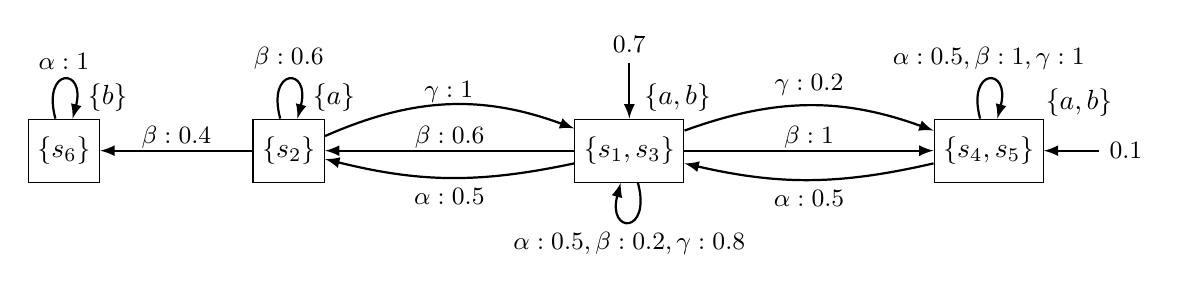
\begin{tikzpicture} [every initial by arrow/.style={thick}]
		\newcommand{\disthor}{90pt}
		\newcommand{\distvert}{110pt}
		%		\createstate{s1}{3,2+4}{$\state_1$};
		
		\node [gstate,initial above,initial text=\small$0.7$,initial distance=20pt] (s13) at (0,0) {$\{\state_1,\state_3\}$};
		\node [gstate,left=\disthor of s13] (s2) {$\{\state_2\}$};
		\node [gstate,initial right,initial text=\small$0.1$,initial distance=20pt,right=\disthor of s13] (s45) {$\{\state_4,\state_5\}$};		
		\node [gstate,left=55pt of s2] (s6) {$\{\state_6\}$};		
		
		\path [trans] (s2) edge node [midway,above=-3pt] {\small$\actionb: 0.4$} (s6);
		\path [trans] (s13) edge node [midway,above=-3pt] {\small$\actionb: 1$} (s45);
		\path [trans] (s13) edge node [midway,above=-3pt] {\small$\actionb: 0.6$} (s2);
		
		\path [trans, bend left=22] (s2) edge node [midway,above=-3pt] {\small$\actionc: 1$} (s13);
		\path [trans,bend left=13] (s13) edge node [midway,below] {\small$\action: 0.5$} (s2);
		
		\path [trans,bend left=20] (s13) edge node [midway,above] {\small$\actionc: 0.2$} (s45);
		\path [trans,bend left=13] (s45) edge node [midway,below] {\small$\action: 0.5$} (s13);
		
		\path [trans] (s2) edge [loop above] node [midway] {\small$\actionb:0.6$} (s2);
		\path [trans] (s13) edge [loop below] node [midway] {\small$\action:0.5,\actionb:0.2,\actionc:0.8$} (s13);
		\path [trans] (s45) edge [loop above=-3pt] node [midway] {\small$\action:0.5, \actionb:1, \actionc:1$} (s45);
		\path [trans] (s6) edge [loop above] node [midway] {\small$\action:1$} (s6);
		
		
		\node [above right=-1pt and -18pt of s13] (ls13) {$\{a,b\}$};
		\node [above right=-1pt and -8pt of s2] (ls2) {$\{a\}$};
		\node [above right=-4pt of s45] (ls45) {$\{a,b\}$};
		\node [above right=-1pt and -8pt of s6] (ls6) {$\{b\}$};
		
		
		
		
	\end{tikzpicture}
\end{document}  
	\caption{\viewNC \view on \chgphN \chgph from Figure \ref{fig:exampleMdp}}
	\label{fig:exampleView}  
\end{figure}
\end{exmp}

\subsection{View Types and Disregarding Views}
In this section we categorize views in two view types. We will present views of two types: binary and categorizing.

\begin{definition}
	\sloppy
	A \viewN \view is called \emph{binary} if for every \chgphN $\chgph = \chgphtuple$ it holds ${\grpfct}[\states] \in \{\{\hasppty, \notppty\}, \{\remelem, \notppty\}, \{\hasppty\, \remelem\}\}$. 
	
	\noindent
	A \viewN \view is called \emph{categorizing} if for every \chgphN $\chgph = \chgphtuple$ it holds $\hasppty, \notppty \notin {\grpfct}[\states]$. 
	\label{def:viewtypes}
\end{definition}

The notion of a binary view is that it maps each state to whether or not it has a certain property. The symbol \hasppty shall be used if it has the property and the symbol \notppty shall be used if it does not have the property. The symbol \remelem can either be used to not group states that have the property or to not group state states that do not have the property. The case of ${\grpfct}[\states] = \{\hasppty, \notppty\}$ may seem of rather little benefit, since the resulting view only contains two states. In the actual implementation such a view might be very useful, as at the tier of visualization there will be the feature of expanding grouped states and show the states they contain. Hence, at runtime it can be decided which states are to be shown, rather than in the phase of preprocessing.

The notion of a categorizing \viewN is that it categorizes states to groups, which have the same value with respect to a certain trait. One could argue that binary \viewsN as well categorize states in two groups that have in common to share having or not having a certain property. We defined categorizing \viewsN as in Definition \ref{def:viewtypes} so that a view either is binary or categorizing to distinguish between the intention of a \viewN.

For binary \viewsN we already presented three cases in which a view is called binary. We will now further elaborate on those cases and generalize the concept and also enable it with categorizing views. When looking at the Elements of the set $\{\{\hasppty, \notppty\}, \{\remelem, \notppty\}, \{\hasppty\, \remelem\}\}$ we observe that for distinct $s,t$ in the set it holds $|s|-|s \; \cap \; t| = 1$, i.e. $s$ and $t$ only differ in one element. We declare the case when $\remelem \in {\grpfct}[\states]$ a special case, because instead of assignment of \hasppty or \notppty, the symbol \remelem is assigned, to avoid grouping on states with this property. In general it may be that states that would be mapped to a certain value should not be grouped. To accomplish this we define disregarding \viewsN.

\begin{definition}
	Let $\chgph = \chgphtuple$ be \achgphN and $\grpfctsub : \smstates \to \imggrp$ a detached grouping function where $\smstates \subseteq \states$. The \viewN $\view^\disregardelements$ is defined by its grouping function $\grpfct^\disregardelements : \states \to \imggrp$ where it is $\grpfctsub^\disregardelements : \smstates \to \imggrp$ with
	\[
	\state \mapsto
	\begin{cases}
		\tilde\grpfct(\state),				& \text{if } \grpfctsub(\state) \notin \{\disregardelements\} \\ 		\remelem,          	& \text{otherwise}
	\end{cases}
	\]
	Its \grpfctN $\grpfct^\disregardelements$ is called \grpfct \emph{disregarding} \disregardelements and the respective \viewN $\view^\disregardelements$ is called \view \emph{disregarding} \disregardelements. 
\end{definition}

With a disregarding \viewN grouping is avoided if its detached \grpfctN would map to any of the values \disregardelements. That is, when reading $\view^\disregardelements$ we know that no grouping occurs on states with one of the properties \disregardelements. In a sense states with these properties are shown - maybe amongst others if $\smstates \subset \states$. For this thesis we will only consider disregarding views for $n = 1$.  
For $n = 1$ $\view$ can be obtained from $\view^\hasppty$ with 
\[
\grpfctsub(\state) = 
\begin{cases}
	\hasppty,				& \text{if } \grpfctsub^\hasppty(\state) = \remelem  \\
	\grpfctsub^\hasppty(\state),       		& \text{otherwise }
\end{cases}
\]
and $\view^\notppty$ from $\view$ with
\[
\grpfctsub^\notppty(\state) = 
\begin{cases}
	\grpfctsub(\state),       		&\text{if } \grpfctsub(\state) = \hasppty  \\ 
	\remelem,				&\text{otherwise } 
\end{cases}
\]

Similarly $\view$ can be obtained from $\view^\notppty$ and $\view^\hasppty$ from $\view$. Hence, for a binary view it suffices to give a Definition for one of $\view^\notppty$, $\view^\hasppty$ and $\view$. Normally we will define binary views as views disregarding \hasppty (i.e. $\view^\hasppty$) and perceive them as filters that show use states that have some property. For categorizing views we wont use disregarding views.

%These have the advantage of being revertible, even if only the detached disregarding \grpfctN is available. This is because if $\grpfctsub^\disregardelem(\state) = \remelem$ we know $\grpfctsub(\state) = \disregardelem$. If $n > 1$ for $\grpfctsub^\disregardelements(\state) = \remelem$ the value $\grpfct(\state)$ is ambigous. When choosing $n = 1$

\subsection{Composition of Views} \label{ch:composition}
In essence views are a simplification generated from \chgphN. It seems rather obvious that the composition of views is a very practical feature, in order to combine simplifications. Therefore, in this chapter we will introduce, formalize and discuss two different notions of compositions. All variants will ensure that the effect caused by each partaking view also takes effect in the composed view. Moreover it is to be generated in a way that the effect of each individual view can be reverted from the composed one.

%\subsubsection{\parllcompNCC} 
The fundamental concept for composition, which we will introduce, is \emph{parallel composition}. Its notion is to group states that match in the function value of all given \grpfctsN. This idea is parallel in the sense that is has no sequential characteristic.

\begin{definition} \label{def:pllcompviewandgfct}
	Let $\view[\viewppty_1], \view[\viewppty_2], \dots, \view[\viewppty_n]$ be \viewsN, and $\grpfct[\viewppty_1], \grpfct[\viewppty_2], \dots, \grpfct[\viewppty_n]$ be their corresponding \grpfctsN. The \grpfctN $\grpfct[{\viewppty_1 \pll \viewppty_2 \pll \dots \pll \viewppty_n}]: \states \to \arbset(\grpfct[\viewppty_1]) \times \dots \times \arbset(\grpfct[\viewppty_n])$ is defined with
	\[
	\state \mapsto (\grpfct[\viewppty_1](\state), \grpfct[\viewppty_2](\state), \dots, \grpfct[\viewppty_n](\state))
	\] 
	and called \emph{parallel composed grouping function}.
	The corresponding parallel composed view is denoted as $\view[\viewppty_1 \pll \viewppty_2 \pll \dots \pll \viewppty_n]$.
\end{definition}

Note that for $\grpfct[{\viewppty_1 \pll \viewppty_2 \pll \dots \pll \viewppty_n}]$ if $\grpfct[\viewppty_1](\state) = \grpfct[\viewppty_2](\state) = \dots = \grpfct[\viewppty_n](\state) = \remelem$ the state \state will not be grouped with any other state due to Definition \ref{def:eqrelview} of \eqrelview. An important property of parallel composed \grpfctsN is, that they defy order. That is, with regard to the impact on the grouping the order of the included \grpfctsN does not matter.

\begin{proposition}
	Let $\grpfct[u]$ and $\grpfct[v]$ be non parallel composed \grpfctsN and \states a set of states. For all $\state_1, \state_2 \in \states$ it holds that
	\[
	\grpfct[u \pll v](\state_1) = \grpfct[u \pll v](\state_2) \iff \grpfct[v \pll u](\state_1) = \grpfct[v \pll u](\state_2)
	\]
\end{proposition}

\begin{proof}
	Let $\grpfct[u]$ and $\grpfct[v]$ be \grpfctsN, $\state_1, \state_2 \in \states$ and
	\begin{align*}
		\grpfct[u \pll v](\state_1) &= (\grpfct[u](\state_1), \grpfct[v](\state_1)) =: (a, b) \\
		\grpfct[u \pll v](\state_2) &= (\grpfct[u](\state_2), \grpfct[v](\state_2)) =: (x, y)			
	\end{align*}
	Then it is
	\begin{align*}
		\grpfct[v \pll u](\state_1) &= (\grpfct[v](\state_1), \grpfct[u](\state_1)) = (b, a) \\
		\grpfct[v \pll u](\state_2) &= (\grpfct[v](\state_2), \grpfct[u](\state_2)) = (y, x)
	\end{align*}
	It follows that
	\[
	\grpfct[u \pll v](\state_1) = \grpfct[u \pll v](\state_2) \iff \grpfct[v \pll u](\state_1) = \grpfct[v \pll u](\state_2)
	\]
	because $(a, b) = (x, y) \iff (a = x) \,\, \land \,\, (b = y) \iff (b, a) = (y, x)$.
\end{proof}

We assume that whenever a \viewN or \grpfctN is parallel composed this is notated as declared in Definition \ref{def:pllcompviewandgfct}. That is, \iffN there is the operator \pll in the subsrcipt of a \viewN or \grpfctN, it is parallel composed. We define the operator \pll in order to construct parallel composed \grpfctsN and \viewsN. 

%\begin{definition}
%	The operator \pll maps two \grpfctsN to a new \grpfctN. It is defined recursively.
%	\begin{enumerate}
%		\item $(\grpfct[\viewppty_1] \pll \grpfct[\viewppty_2])(\state) := (\grpfct[\viewppty_1](\state),\grpfct[\viewppty_2](\state)) = \grpfct[\viewppty_1 \pll \viewppty_2](\state)$ \\
%		if it is not $\grpfct[\viewppty_1] = \grpfct[x] \pll \grpfct[y]$ or $\grpfct[\viewppty_2] = \grpfct[x] \pll \grpfct[y]$ for some \grpfctsN \grpfct[x], \grpfct[y].
%		\item $((\grpfct[\viewppty_1], \dots, \grpfct[\viewppty_n]) \pll \grpfct[\viewppty])(\state) := (\grpfct[\viewppty_1](\state), \dots, \grpfct[\viewppty_n](\state), \grpfct[\viewppty](\state)) = \grpfct[{\viewppty_1 \pll \viewppty_2 \pll \dots \pll \viewppty_n \pll \viewppty}](\state)$ 
%		\\ if for all $i \in \{1, \dots, n\}$ it is not $\grpfct[\viewppty_i] = \grpfct[x] \pll \grpfct[y]$ and also not $\grpfct = \grpfct[x] \pll \grpfct[y]$ for some \grpfctsN \grpfct[x], \grpfct[y].
%	\end{enumerate}
%	
%\end{definition}
\begin{definition}
	The operator \pll maps two \grpfctsN to a new \grpfctN. It is defined inductively.
	\begin{enumerate}
		\item $(\grpfct[\viewppty_1] \pll \grpfct[\viewppty_2])(\state) := \grpfct[{\viewppty_1 \pll \viewppty_2}](\state)$
		\item $(\grpfct[{\viewppty_1 \pll \dots \pll \viewppty_n}] \pll \grpfct)(\state) := \grpfct[{\viewppty_1 \pll \dots \pll \viewppty_n \pll \viewppty}](\state)$ \quad where $n \in \natnums$
		\item $(\grpfct \pll \grpfct[{\viewppty_1 \pll \dots \pll \viewppty_n}])(\state) := \grpfct[{\viewppty \pll \viewppty_1 \pll \dots \pll \viewppty_n}](\state)$ \quad where $n \in \natnums$
	\end{enumerate}
	
\end{definition}

\begin{proposition}
	The operator \pll is associative.
\end{proposition}

\begin{proof}
	Let	$\grpfct[\viewppty_1], \grpfct[\viewppty_2], \grpfct[\viewppty_3]$ be \grpfctsN. For simplicity we omit the parameter (state \state).
	\[
		\grpfct[\viewppty_1] \pll (\grpfct[\viewppty_2] \pll \grpfct[\viewppty_3]) = \grpfct[\viewppty_1] \pll \grpfct[{\viewppty_2 \pll \viewppty_3}] = \grpfct[{\viewppty_1 \pll \viewppty_2 \pll \viewppty_3}] = \grpfct[{\viewppty_1 \pll \viewppty_2}] \pll \grpfct[\viewppty_3] = (\grpfct[\viewppty_1] \pll \grpfct[\viewppty_2]) \pll \grpfct[\viewppty_3]
	\]
	The proof is analogous if one or several of the \grpfctsN are parallel composed.
	
%	(\grpfct[\viewppty_1](\state) \pll (\grpfct[\viewppty_2](\state) \pll \grpfct[\viewppty_3]))(\state) = \grpfct[\viewppty_1](\state) \pll \grpfct[{\viewppty_2 \pll \viewppty_3}](\state) = \grpfct[{\viewppty_1 \pll \viewppty_2 \pll \viewppty_3}] = \grpfct[{\viewppty_1 \pll \viewppty_2}](\state) \pll \grpfct[\viewppty_3](\state) = (\grpfct[\viewppty_1](\state) \pll \grpfct[\viewppty_2])(\state) \pll \grpfct[\viewppty_3](\state)
\end{proof}

We write $\view[\viewppty_1] \pll \view[\viewppty_2]$ for $\view[\viewppty_1 \pll \viewppty_2]$ defined by the \grpfctN $\grpfct[\viewppty_1] \pll \grpfct[\viewppty_2] = \grpfct[\viewppty_1 \pll \viewppty_2]$.
%The operator \pll used in the definition is inspired from the operator used in electric circuits, when the respective elements are connected in parallel. 
%If we want to speak about this grouping function in a general way, where it is only of importance that we refer to this type of composition and the given \grpfctsN are of no importance, we will denote a \emph{\parllcompN \grpfctN} with \gfctpll.
%
%The operator \pll in \gfctpll is associative with respect to the grouped states. That is exactly the same states are grouped no matter where parenthesis are put.
%\begin{proposition}
%	Let $\grpfct[u], \grpfct[v], \grpfct[w]$ be \grpfctsN and \states a set of states. For all $\state_1, \state_2 \in \states$ it holds that
%	\[
%	\grpfct[(u \pll v) \pll w](\state_1) = \grpfct[(u \pll v) \pll w](\state_2) \iff \grpfct[u \pll (v \pll w)](\state_1) = \grpfct[u \pll (v \pll w)](\state_2)
%	\]
%\end{proposition}
%
%\begin{proof}
%Let $\grpfct[u], \grpfct[v], \grpfct[w]$ be \grpfctsN and \states a set of states with $\state \in \states$. It is
%\begin{equation*}
%	\begin{aligned}[c]
%			&\grpfct[u \pll v](\state) = (\grpfct[u](\state), \grpfct[v](\state)) \\
%			&\grpfct[(u \pll v) \pll w](\state) = ((\grpfct[u](\state), \grpfct[v](\state)), \grpfct[w](\state))
%		\end{aligned}
%	\quad\quad\quad\quad\quad
%	\begin{aligned}[c]
%			&\grpfct[v \pll w](\state) = (\grpfct[v](\state), \grpfct[w](\state)) \\
%			&\grpfct[u \pll (v \pll w)](\state) = (\grpfct[u](\state), (\grpfct[v](\state), \grpfct[w](\state))\\
%		\end{aligned}					
%\end{equation*}
%\\
%\noindent
%Let $\state_1, \state_2 \in \states$ be arbitrary. Moreover let %$\grpfct[((u \pll v) \pll w)](\state_1) =: ((a,b),c)$ and $\grpfct[u \pll (v \pll w)](\state_1) =: ((x, y), z)$, then $\grpfct[u \pll (v \pll w)](\state_1) = (a, (b, c))$ and $\grpfct[u \pll (v \pll w)](\state_2) = (x, (y, z))$
%\begin{equation*}
%	\begin{aligned}[c]
%			&\grpfct[(u \pll v) \pll w](\state_1) =: ((a,b),c) \text{ and} \\
%			&\grpfct[(u \pll v) \pll w](\state_2) =: ((x, y), z) \text{.}
%		\end{aligned}
%	\quad\quad\text{Then it is}\quad\quad
%	\begin{aligned}[c]
%			&\grpfct[u \pll (v \pll w)](\state_1) = (a, (b, c)) \text{ and} \\
%			&\grpfct[u \pll (v \pll w)](\state_2) = (x, (y, z)).
%		\end{aligned}
%	\quad\quad\quad				
%\end{equation*}
%
%\noindent
%Then it is
%\[
%	\grpfct[(u \pll v) \pll w](\state_1) = \grpfct[(u \pll v) \pll w](\state_2) \iff \grpfct[u \pll (v \pll w)](\state_1) = \grpfct[u \pll (v \pll w)](\state_2)
%\]
%
%\noindent
%This is because
%\begin{align*}
%	&((a, b), c) = ((x, y), z) \\
%	\iff \quad &(a, b) = (x, y) \land c = z \\
%	\iff \quad &a = x \land b = y \land c = z \\
%	\iff \quad &a = x \land (b, c) = (y, z) \\
%	\iff \quad &(a, (b, c)) = (x, (y, z))
%\end{align*}
%\end{proof}
%
%Note that the operator \pll is not associative, because it is not defined for expressions of the form $\grpfct[\viewppty] \pll (\grpfct[\viewppty_1], \dots, \grpfct[\viewppty_n])$. For the same reason \pll is in general not commutative (only for the base case). These are no issues since parallel composed \grpfctsN defy order. 
Note that the operator \pll is obviously not commutative, but as parallel composed \grpfctsN defy order, the absence of this property will not have any effect on the resulting grouping.

\begin{definition}
	Let $\grpfct[\viewppty_1 \pll \dots \pll \viewppty_n]$ be a parallel composed grouping function. The operator \pllrev is defined as
	\[
	\grpfct[\viewppty_1, \dots, \viewppty_n] \pllrev \grpfct[\viewppty_i] := (\grpfct[\viewppty_1], \dots, \grpfct[\viewppty_{i-1}],\grpfct[\viewppty_i+1], \dots, \grpfct[n]) = \grpfct[\viewppty_1 \pll \dots \pll \viewppty_{i-1} \pll \viewppty_{i+1} \pll \dots \pll \viewppty_n]
	\]
\end{definition}

The operator \pllrev is the reversing operator to \pll. Given a parallel composed view and an in it contained grouping function, it removes this view. We write $\view[\viewppty_1 \pll \dots \pll \viewppty_n] \pllrev \view[\viewppty_i]$ for the view defined by the \grpfctN $\grpfct[\viewppty_1 \pll \dots \pll \viewppty_{i-1} \pll \viewppty_{i+1} \pll \dots \pll \viewppty_n]$.

%\subsubsection{Selective Composition} \label{subsec:selecitvecomp}
A variant of parallel composition is \emph{selective composition}. It aims for application of the grouping function only on certain states, where the other composing functions have a certain value.



\begin{definition}
	Let $\view[\viewppty_1 \pll \dots \pll 
	\viewppty_n]$ be a parallel composed view with its \grpfctN $\grpfct[{\viewppty_1 \pll \dots \pll \viewppty_n}]$, where $n$ might be 1 and let \view be another view with its \grpfctN \grpfct. We write $\imggrp_i$ for the image of $\grpfct[\viewppty_i]$.
	Given a set $\compselectset \subseteq \{ (\grpfct[\viewppty_i], a) \mid a \in \imggrp_i, i \in \{1, \dots, n\}\}$ the operator \compselectpure is defined as $\grpfct[{\viewppty_1 \pll \dots \pll \viewppty_n}] \compselect \grpfct := \grpfct[{\viewppty_1 \pll \dots \pll \viewppty_n} \pll \viewppty]: \states \to \arbset$ with
	\[
	\state \mapsto
	\begin{cases}
		(\grpfct[\viewppty_1](\state), \dots, \grpfct[\viewppty_n](\state),  \grpfct[\viewppty](\state))				& \text{if } \forall i \in \{1, \dots, n\} : (\grpfct[\viewppty_i], \grpfct[\viewppty_i](\state)) \in \compselectset \\ 		
		(\grpfct[\viewppty_1](\state), \dots, \grpfct[\viewppty_n](\state),  \remelem),          	& \text{otherwise}
	\end{cases}
	\]
\noindent
Then $\view[\viewppty_1 \pll \dots \pll 
\viewppty_n \pll \viewppty]$ is a parallel composed \viewN with $\grpfct[{\viewppty_1 \pll \viewppty_2 \pll \dots \pll \viewppty_n} \pll \viewppty]$ being its parallel composed \grpfctN.
%\label{def:compositionselective}
\end{definition}
The set \compselectset determines on which states the \viewN \view shall take effect. For instance, $\compselectset = \{(\grpfct[\viewppty_1], a_1),(\grpfct[\viewppty_1], b_1), (\grpfct[\viewppty_2], a_2)\}$ induces that \view only takes effect on a state \state if 
\[
((\grpfct[\viewppty_1](\state) = a_1) \lor (\grpfct[\viewppty_1](\state) = b_1)) \land (\grpfct[\viewppty_2](\state) = a_2)
\]
That is, if this boolean expression is false, the last entry in the tuple is \remelem and only otherwise it is $\grpfct(\state)$.

%\begin{definition}
%	Let $\view[\viewppty_1 \pll \viewppty_2 \pll \dots \pll 
%	\viewppty_n]$ be a parallel composed view with its \grpfctN $\grpfct[{\viewppty_1 \pll \viewppty_2 \pll \dots \pll \viewppty_n}]$, where $n$ might be 1 and let \view be another view with its \grpfctN \grpfct. 
%	We write $\imggrp_i$ for the image of $\grpfct[\viewppty_i]$. 
%	Given a set $\compselectset \subseteq \{ (\grpfct[\viewppty_i], a) \mid a \in \imggrp_i, i \in \{1, \dots, n\}\}$ the operator \compselectpure is defined as $\grpfct[{\viewppty_1 \pll \viewppty_2 \pll \dots \pll \viewppty_n}] \compselect \grpfct := \grpfct[{\viewppty_1 \pll \viewppty_2 \pll \dots \pll \viewppty_n} \pll \viewppty]: \states \to \arbset$ with
%	\[
%	\state \mapsto (\grpfct[\viewppty_1](\state), \dots, \grpfct[\viewppty_n]'(\state))
%	\]
%	where $\grpfct' : \states \to \imggrp$ with $\grpfctsub' : \smstates \to \imggrp, \state \to \grpfct(\state)$ and $\smstates := \{\state \in \states \mid \forall i \in \{1, \dots, n\} : (\grpfct[\viewppty_i], \grpfct[\viewppty_i](\state)) \in \compselectset\}$.
%	
%	
%	
%	\noindent
%	Then $\view[\viewppty_1 \pll \dots \pll 
%	\viewppty_n \pll \viewppty]$ is a parallel composed \viewN with $\grpfct[{\viewppty_1 \pll \dots \pll \viewppty_n} \pll \viewppty]$ being its parallel composed \grpfctN.
%	\label{def:compositionselective}
%\end{definition}
%
%The set \compselectset determines on which states the \viewN \view shall take effect, by restricting the state set \smstates of the detached grouping function to those states, that meet the requirement. Every state that is not in \smstates then by Definition \ref{def:grpfct} is mapped to \remelem. Considering $\compselectset = \{(\grpfct[\viewppty_1], a_1),(\grpfct[\viewppty_1], b_1), (\grpfct[\viewppty_2], a_2)\}$ it induces that \view only takes effect on a state \state of \mdp if 
%
%\[
%	((\grpfct[\viewppty_1](\state) = a_1) \lor (\grpfct[\viewppty_1](\state) = b_1)) \land (\grpfct[\viewppty_2](\state) = a_2)
%\]
%
%That is, if this boolean expression is false the last entry in the mapped tuple in Definition \ref{def:compositionselective} equals \remelem and only otherwise equals $\grpfct(\state)$. Note that Definition \ref{def:compositionselective} is the same as declaring $\grpfct[{\viewppty_1 \pll \viewppty_2 \pll \dots \pll \viewppty_n}] \compselect \grpfct$ through $\grpfct[{\viewppty_1 \pll \viewppty_2 \pll \dots \pll \viewppty_n} \pll \viewppty]: \states \to \arbset$ with
%\[
%\state \mapsto
%\begin{cases}
%	(\grpfct[\viewppty_1](\state), \dots, \grpfct[\viewppty_n](\state),  \grpfct[\viewppty](\state))				& \text{if } \forall i \in \{1, \dots, n\} : (\grpfct[\viewppty_i], \grpfct[\viewppty_i](\state)) \in \compselectset \\ 		
%	(\grpfct[\viewppty_1](\state), \dots, \grpfct[\viewppty_n](\state),  \remelem),          	& \text{otherwise}
%\end{cases}
%\]
%In the original definition the set of states \smstates is restricted which causes the remaining elements to be mapped to \remelem. In the equivalent proposed definition here the grouping function is applied only if the requirement is met and otherwise the element \remelem is mapped. Hence, the effect is the same: Whenever the requirement is met the last entry of the tuple is $\grpfct(\state)$ otherwise it is \remelem. Although the latter proposed definition may seem more intuitive the the actual Definition \ref{def:compositionselective} was chosen because it matches the implementation better.


\end{document}

